\documentclass[letterpaper,12pt]{article}
\usepackage{matharticle}
\usepackage{graphtheory}
\usepackage{flowchart}
\usepackage{afterpage}
\usepackage{url}
\usepackage{graphicx}
\usetikzlibrary{arrows}
\pagestyle{plain}
\newcommand{\sR}{\mathscr{R}}
\newcommand{\coloring}[1]{\(#1\)-coloring}
\newcommand{\colorable}[1]{\(#1\)-colorable}
\newcommand{\chromatic}[1]{\(#1\)-chromatic}
\newcommand{\X}{\chi}
\renewcommand{\d}{\delta}
\newcommand{\D}{\Delta}
\renewcommand{\l}{\lambda}
\newcommand{\SG}{\mathscr{G}}
\newcommand{\BO}{\mathcal{O}}
\newtheorem{proposition}{Proposition}
\newtheorem{axiom}{Axiom}
\newcommand{\restrict}[2]{#1\raise-0.5ex\hbox{\ensuremath|}_{#2}}
\newcommand{\FR}{\text{FR}}
\newcommand{\DP}{\text{DP}}
\allowdisplaybreaks
\begin{document}

\title{Determining a Graph's Chromatic Number for Part Consolidation in Axiomatic Design}
\author{Jeffery A. Cavallaro\\
  Graduate Student\\
  Mathematics Department\\
  San Jose State University\\
  \url{jeffery.cavallaro@sjsu.edu}}

\maketitle

\section{Axiomatic Design}\label{sec:axiomatic}

The axiomatic design (AD) framework was developed in the late \(20^{th}\)-century by Professor Nam P. Suh while at
MIT and NSF~\cite{suh}.  This was in response to concern in the engineering community that \emph{design} was
being practiced almost exclusively as an ad hoc creative endeavor with very little in the way of scientific
discipline.  In the words of Professor Suh:
\begin{quote}
  \vspace{-\baselineskip}
  It [design] might have preceded the development of natural sciences by scores of centuries.  Yet, to this day,
  design is being done intuitively as an art.  It is one of the few technical areas where experience is more
  important than formal education~\cite{suh}.
\end{quote}
Professor Suh was not making these claims in an educational vacuum, but in the shadow of several recent major
design failures such as the Union Carbide plant disaster in India, nuclear power plant accidents at Three Mile
Island and Chernobyl, and the Challenger space shuttle O-ring failure.  Furthermore, Professor Suh asserts that
design-related issues resulting in production problems and operating failures were increasingly occurring in
everything from consumer products to big-ticket items.  As a result, AD has been widely adopted by companies to
promote efficiency and accuracy in the design process, resulting in more reliable products and reduced
manufacturing costs~\cite{shirwaiker}.

The following sections provide an overview of axiomatic design as specified in detail by Professor
Suh~\cite{suh,suh2}, and summarized by Behdad et al.~\cite{cavallaro,jahanbekam}.  Following the overview is a
description of how an algorithm like the algorithm proposed by this research can be a helpful tool to a designer
using the AD framework.

\subsection{Design}\label{sec:sub:design}

\emph{Design} is defined as the process by which it is determined \emph{what} needs to be achieved and then
\emph{how} to achieve it.  Thus, the decisions on what to do are just as important as the decisions on how to do
it.  \emph{Creativity} is the process by which experience and intuition are used to generate solutions to perceived
needs.  This includes pattern matching to and adapting existing solutions and synthesizing new solutions.  Thus,
creativity plays a vital role in design.  Different designers may approach the same problem differently, and their
varying levels of creativity may lead to very different, yet still plausible, solutions.  Therefore, there needs to
be a design-agnostic method for comparing different designs with the goal of selecting the best one.

This discussion will sound familiar to mathematicians, since creativity is a very important part of solving math
problems, particularly in the writing of proofs.  Thus, the field of mathematics has established various tests on
what constitutes a good proof.  For example:
\begin{itemize}
\item Does every conclusion result by proper implication from existing definitions, axioms, and previously proved
  conclusions?
\item Is direct proof, contrapositive proof, proof by contradiction, or proof by induction the best approach for a
  particular problem?
\item Do proofs by induction contain clear basic, assumptive, and inductive steps?
\item Are all subset and equality relationships properly proved via membership implication?
\item Are all necessary cases included and stated in a mutually exclusive manner?
\item Are degenerate cases sufficiently highlighted?
\item Are all equivalences proved in a proper circular fashion?
\item Are key and reused conclusions highlighted in lemmas?
\end{itemize}
In short, Professor Suh was looking for a similar framework for the more general concept of design.

\subsection{The Axiomatic Design Framework}\label{sec:sub:framework}

The \emph{best} design among a set of candidates is the design that exactly satisfies a clearly defined set of
needs and has the greatest probability of success in meeting those needs.  In a desire not to hinder the creative
element needed for design, yet provide some methodology to distinguish bad designs from good designs from better
designs, the diagram in \figurename~\ref{fig:design} establishes the overall framework for axiomatic design.

\begin{figure}[H]
  \centering
  \scalebox{0.75}{
    \begin{tikzpicture}[>=latex',every text node part/.style={align=center}]
      \node (cn) [draw,terminal] at (0,0) {customer \\[-2ex] needs};
      \node (pd) [draw,process,right=of cn] {problem \\[-2ex] definition};
      \node (cp) [draw,process,right=2cm of pd] {creative \\[-2ex] process};
      \node (ap) [draw,process,right=2cm of cp] {analytical \\[-2ex] process};
      \node (uc) [draw,process,right=of ap] {ultimate \\[-2ex] check};
      \node (fd) [draw,terminal,right=of uc] {final \\[-2ex] design};
      \draw [->] (cn) -- (pd);
      \draw [->] (pd) -- node [auto] {FRs} (cp);
      \draw [->] (cp) -- node [auto] {candidate \\[-2ex] design} (ap);
      \draw [->] (ap) -- (uc);
      \draw [->] (uc) -- (fd);
      \draw [->] (ap) -- ($(ap) + (0,-1.5cm)$) -| (cp);
    \end{tikzpicture}
  }
  \caption{The axiomatic design framework.}
  \label{fig:design}
\end{figure}

Design starts with the desire to satisfy a set of precisely stated \emph{customer needs}.  The term \emph{customer}
refers to any entity that expresses needs, and can be as varied as individuals, organizations, or society.  In the
\emph{problem definition} phase, the designer determines how the customer needs will be met by generating a minimal
list of \emph{functional requirements} (FRs) that directly and exclusively fulfill the needs.  It is this list of
FRs that determines exactly \emph{what} is to be accomplished.

Once the set of FRs has been determined, the designer begins the \emph{creative process} by mapping the FRs into
solutions that are embodied in so-called \emph{design parameters} (DPs).  The DPs contain all of the information
concerning \emph{how} the various FRs are to be satisfied: parts lists, drawings, specifications, etc.  The FRs
exist in a design-agnostic \emph{functional space} and the {\DP}s exist in a solution-specific \emph{physical
  space}.  It is the designer's job to provide the most efficient mapping between the two spaces.  This process is
represented by \figurename~\ref{fig:mapping}.

\begin{figure}[H]
  \centering
  \begin{tikzpicture}[>=latex',every text node part/.style={align=center}]
    \node (fs) [draw,cloud] at (0,0) {FR1 \\ FR2 \\ FR3 \\ \vdots};
    \node [below=1ex of fs] {functional \\ space};
    \node (ps) [draw,cloud,right=1.5in of fs] {DP1 \\ DP2 \\ DP3 \\ \vdots};
    \node [below=1ex of ps] {physical \\ space};
    \draw [->] (fs) to [bend left=45] (ps);
    \draw [->] (fs) to [bend left=30] (ps);
    \draw [->] (fs) to [bend right=30] (ps);
    \draw [->] (fs) to [bend right=45] (ps);
    \draw [->] (fs) -- node [auto] {mapping} (ps);
  \end{tikzpicture}
  \caption{Mapping FRs to DPs.}
  \label{fig:mapping}
\end{figure}

Simple problems may require only one level of FRs; however, more complicated designs may require a hierarchial
structure of FRs from more general to more detailed requirements.  This type of design is often referred to as
\emph{top-down} design.  Each individual FR layer has its own DP mapping.  In fact, the mapping process on one
level should be completed prior to determining the FRs for the next level.  This is because DP choices on one level
may affect requirements on the next level.  For example, consider a FR related to a moving part in a design.  The
DP for this FR could specify that the part be moved either manually or automatically.  Each choice would result in
different FRs for the actual mechanism selected by the DP.

The FR/DP mapping at each level in the design hierarchy is described by the \emph{design equation}, which is shown
in \equationname~\ref{eqn:design}.
\begin{equation}
  \label{eqn:design}
  [\FR]=[\text{A}][\DP]
\end{equation}
The design equation is a matrix equation that maps a vector of \(m\) FRs to a vector of \(n\) DPs via an \(m\times
n\) design matrix A.  As will be shown later in this section, good designs require \(m=n\).  A full discussion of
the design matrix element values is well beyond the scope of this research.  Instead, the following two summary
values are used:
\[A_{ij}=\begin{cases}
X, & \FR_i\ \text{depends on}\ \DP_j \\
0, & \FR_i\ \text{does not depend on}\ \DP_j
\end{cases}\]

Since the FR/DP mapping is non-unique, there needs to be a method to compare different plausible designs so that
the best design can be selected as the final design.  Thus, the framework in \figurename~\ref{fig:design} includes
an \emph{analytical process}, where designs are judged by a set of axioms, corollaries, and theorems that specify
the properties common to all good designs.  Once the best design, according to this analysis, is selected, it
undergoes an \emph{ultimate check} to make sure that it exactly meets all of the customer's needs.  If so, then
that design is selected as the final design.

\subsection{The Axioms}\label{sec:sub:axioms}

The analytical process is based on two main axioms: the independence axiom and the information axiom.  This section
describes these axioms and their related corollaries and theorems.

The independence axiom~\cite{suh} imposes a restriction on the FR/DP mapping:

\begin{axiom}[The Independence Axiom]
  \label{axm:independence}
  An optimal design always maintains the independence of the FRs.  This means that the FRs and DPs are related in
  such a way that a specific DP can be adjusted to satisfy its corresponding FR without affecting other FRs.
\end{axiom}

The ideal case is when the design matrix is a diagonal matrix and so each FR is mapped to and is satisfied by
exactly one DP.  This is referred to as an \emph{uncoupled} design, which is demonstrated in
\figurename~\ref{fig:uncoupled}.  Uncoupled designs completely adhere to the independence axiom.

\begin{figure}[H]
  \begin{equation*}
    \begin{bmatrix}
      \FR1 \\ \FR2 \\ \FR3
    \end{bmatrix}=\begin{bmatrix}
    X & 0 & 0 \\
    0 & X & 0 \\
    0 & 0 & X
    \end{bmatrix}\begin{bmatrix}
      \DP1 \\ \DP2 \\ \DP3
    \end{bmatrix}
  \end{equation*}
  \vspace{-\baselineskip}
  \caption{An example of an uncoupled design.}
  \label{fig:uncoupled}
\end{figure}

The next best situation is when the design matrix is a lower-triangular matrix.  The idea is to finalize the first
DPs before moving on to the later DPs.  Thus, \(\text{DP}_i\) can be adjusted without affected \(\FR_1\) through
\(\FR_{i-1}\).  This is referred to as a \emph{decoupled} design, which is demonstrated in
\figurename~\ref{fig:decoupled}.  Although decoupled designs do not completely adhere to the independence axiom,
they may be reasonable compromises in designs that address complex problems.

\begin{figure}[H]
  \begin{equation*}
    \begin{bmatrix}
      \FR1 \\ \FR2 \\ \FR3
    \end{bmatrix}=\begin{bmatrix}
    X & 0 & 0 \\
    X & X & 0 \\
    X & X & X
    \end{bmatrix}\begin{bmatrix}
      \DP1 \\ \DP2 \\ \DP3
    \end{bmatrix}
  \end{equation*}
  \vspace{-\baselineskip}
  \caption{An example of a decoupled design.}
  \label{fig:decoupled}
\end{figure}

The worst solution is a non-triangular matrix, where every change in a DP affects multiple FRs in an unconstrained
fashion.  This is referred to as a \emph{coupled} design, which is demonstrated in \figurename~\ref{fig:coupled}.
Coupled designs are in complete violation of the independence axiom and generally should be decoupled by reworking
the FRs or by adding additional DPs.

\begin{figure}[H]
  \begin{equation*}
    \begin{bmatrix}
      \FR1 \\ \FR2 \\ \FR3
    \end{bmatrix}=\begin{bmatrix}
    X & X & X \\
    X & X & X \\
    X & X & X
    \end{bmatrix}\begin{bmatrix}
      \DP1 \\ \DP2 \\ \DP3
    \end{bmatrix}
  \end{equation*}
  \vspace{-\baselineskip}
  \caption{An example of a coupled design.}
  \label{fig:coupled}
\end{figure}

Unfortunately, adding additional DPs runs counter to the second axiom: the information axiom~\cite{suh}.

\begin{axiom}[The Information Axiom]
  The best design is an uncoupled design that has the minimum information content.
\end{axiom}

The amount of \emph{information} contained in a particular DP is inversely related to the probability that the DP
can successfully satisfy its corresponding FR(s) by \equationname~\ref{eqn:info}.
\begin{equation}
  \label{eqn:info}
  I=\log_2\left(\frac{1}{p}\right)
\end{equation}
where \(p\) is the probability of success and \(I\) is measured in bits.  This probability must take into
consideration such things as tolerances, ease of manufacture, and failure rates.  The information content of a
design is then the sum of the information content of its individual DPs.

From these two axioms come the following seven corollaries~\cite{suh}:
\begin{corollary}
  \label{cor:decouple}
  Decouple or separate parts or aspects of a solution if the FRs are coupled or become interdependent in the
  designs proposed.
\end{corollary}
\begin{corollary}
  \label{cor:minfrs}
  Minimize the number of FRs.
\end{corollary}
\begin{corollary}
  \label{cor:integrate}
  Integrate design features in a single physical part if FRs can be independently satisfied in the proposed
  solution.
\end{corollary}
\begin{corollary}
  \label{cor:standard}
  Use standardized or interchangeable parts if the use of these parts is consistent with the FRs.
\end{corollary}
\begin{corollary}
  \label{cor:shapes}
  Use symmetrical shapes and/or arrangements if they are consistent with the FRs.
\end{corollary}
\begin{corollary}
  \label{cor:tolerance}
  Specify the largest allowable tolerance in stating FRs.
\end{corollary}
\begin{corollary}
  \label{cor:uncoupled}
  Seek an uncoupled design that requires less information than coupled designs in satisfying a set of FRs.
\end{corollary}

The theorems that arise from these axioms and corollaries are used to prove that an optimal design results from a
square design matrix.  In other words, the number of FRs should be equal to the number of DPs.  First, consider the
case where there are more FRs than DPs.  This forces a single DP to be mapped to multiple FRs.  Otherwise, some FRs
cannot be satisfied by the DPs.  This result is stated in \theoremname~\ref{thm:frgtdp}~\cite{suh}.

\begin{theorem}
  \label{thm:frgtdp}
  When the number of DPs is less that the number of FRs, either a coupled design results or the FRs cannot be
  satisfied.
\end{theorem}

A possible solution to this problem is given by \theoremname~\ref{thm:adddp}~\cite{suh}.
\begin{theorem}
  \label{thm:adddp}
  A coupled design due to more FRs than DPs can be decoupled by adding new DPs if the additional DPs result in a
  lower triangular design matrix.
\end{theorem}

An example is show in \figurename~\ref{fig:dcexample}.  Note that the addition of DP3 results in a decoupled design.

\begin{figure}[H]
  \[\begin{bmatrix}
  \FR1 \\ \FR2 \\ \FR3
  \end{bmatrix}=\begin{bmatrix}
  X & 0 \\
  X & X \\
  X & X \\
  \end{bmatrix}\begin{bmatrix}
    \DP1 \\ \DP2 \\
  \end{bmatrix}\implies\begin{bmatrix}
  \FR1 \\ \FR2 \\ \FR3
  \end{bmatrix}=\begin{bmatrix}
  X & 0 & 0 \\
  X & X & 0 \\
  X & X & X \\
  \end{bmatrix}\begin{bmatrix}
    \DP1 \\ \DP2 \\ \DP3
  \end{bmatrix}\]
  \vspace{-\baselineskip}
  \caption{Decoupling a design by adding DPs.}
  \label{fig:dcexample}
\end{figure}

Next, consider the case where the number of FRs is less than the number of DPs.  Assuming that the design is not
coupled, this means that either a DP exists that does not address any FRs or multiple DPs exist that address a
single FR and hence can be integrated into a single DP.  Such a design is called a \emph{redundant} design.  This
is addressed by \theoremname~\ref{thm:frltdp}~\cite{suh}.

\begin{theorem}
  \label{thm:frltdp}
  When there are less FRs than DPs then the design is either coupled or redundant.
\end{theorem}

Finally, the previous three theorems lead to the conclusion in \theoremname~\ref{thm:freqdp}~\cite{suh}.

\begin{theorem}
  \label{thm:freqdp}
  In an ideal design, the number of FRs is equal to the number of DPs.
\end{theorem}

\subsection{Part Consolidation}\label{sec:sub:parts}

One particularly important design parameter is the number of parts in a product design.  According to Professor
Suh:
\begin{quote}
  \vspace{-\baselineskip}
  Poorly designed products often cost more because they use more materials or parts than do well-designed products.
  They are often difficult to manufacture and maintain~\cite{suh}.
\end{quote}
Decreasing the number of parts in a design while maintaining the independence of the FRs is consistent with
\corollaryname~\ref{cor:integrate} and lowers the information content of the design.  In fact, Tang, et
al.~\cite{tang} describe how part consolidation reduces the weight and complexity of a final product while boosting
reliability and reducing cost.

An informative example of part consolidation is the combination can/bottle opener shown in
\figurename~\ref{fig:opener}.  The design of this handy utensil has two FRs that are consolidated into a single
part, yet remain independent as long as there is no desire to open a can and a bottle simultaneously (although that
would be a popular trick around a campfire).

\begin{figure}[H]
  \centering
  \includegraphics{opener}

  \bigskip

  \begin{tabular}{|c|l|}
    \hline
    FR1 & Open beverage cans \\
    \hline
    FR2 & Open beverage bottles \\
    \hline
  \end{tabular}
  \caption{A part consolidation example.}
  \label{fig:opener}
\end{figure}

\subsection{Research Goals}\label{sec:sub:goals}

The primary goal of this research is to provide designers with a tool that they can use to determine the minimum
number of parts required to realize a particular design at a particular level in a FR/DP hierarchy.  The designer
is required to construct a graph whose vertices are the FRs and whose edges indicate that the endpoint FRs need to
be realized by separate parts due to various design constraints.  How these edges are actually determined is beyond
the scope of this research.  Nonadjacent FRs are candidates for part consolidation.  The goal is to find the
chromatic number of the resulting graph, which corresponds to the minimum number of parts required for the
candidate design.

To be a viable tool, an algorithm running as a computer program must be able to deliver an answer in a reasonable
amount of time.  Unfortunately, finding the chromatic number of a graph is known to be an inherently intractable
problem~\cite{garey}.  The nature of such problems is discussed in \sectionname~\ref{sec:problems}, but for now
this is taken to mean that the time required to find a solution grows exponentially with the number of vertices in
the graph.  Furthermore, although not fully proven, it appears likely that there is no way to do any better than an
exponential-time solution.  Therefore, it is necessary to apply some solution parameters:
\begin{enumerate}
\item Maximum number of FRs in a design graph.
\item Target edge density in a design graph.
\item Acceptable runtime duration to obtain a solution.
\end{enumerate}

Determining solid requirements for the maximum number of FRs and the target edge density would require a full case
study by a qualified mechanical engineer; however, the examples submitted by our colleagues at SUNY, Buffalo all
have under \(20\) FRs with low to average edge density.  These values seem reasonable: designs with too many FRs
may become untenable and hence broken up into multiple layers in the design hierarchy and designs with too many
edges may be too coupled.  Although acceptable duration time is subjective, a limit of about one minute will be
selected as the goal.

Thus, the primary goal of this research is to provide AD designers with a tool that can determine the minimum
number of parts needed to realize a particular design having about \(20\) FRs and less than \(50\%\) edge density
in less than one minute.  Designs with different minimum parts requirements can then be compared during the
analytical process phase of the axiomatic design as part of the overall process of selecting the best design.  Of
course, this tool will be an algorithm that can be run on a computer.

This research compares the two most well-known existing algorithms for determining the chromatic number of a graph:
the Christofides algorithm~\cite{christofides} with improvements by Wang~\cite{wang} and the Zykov
algorithm~\cite{corneil}.  A new algorithm is then proposed that is a modification of the Zykov algorithm with the
goal of outperforming the existing algorithms.

\section{Graph Theory}

This section presents the concepts, definitions, and theorems from the field of graph theory that are needed in the
development of the two algorithms.  This material is primarily taken from the textbooks used \cite{chartrand} and
class notes compiled by the author during his undergraduate and graduate graph theory classes at SJSU.

\subsection{Simple Graphs}

The problem of part consolidation is best served by a class of graphs called \emph{simple graphs}:

\begin{definition}[Simple Graph]
  A \emph{simple graph} is a mathematical object represented by a tuple \(G=(V,E,\ldots)\) consisting of a
  non-empty and finite set of \emph{vertices} (also called \emph{nodes}) \(V(G)\), a finite and possibly empty set
  of edges \(E(G)\), and zero of more relations.  Each edge is represented by a two-element subset of \(V(G)\)
  called the \emph{endpoints} of the edge:
  \[E(G)\subseteq\ps_2\left(V(G)\right)\]
  Each relation has \(V(G)\) or \(E(G)\) as its domain and is used to associated vertices or edges with
  problem-specific attributes.
\end{definition}

For the remainder of this work, the use of the term ``graph'' implies a ``simple graph.''

The choice of two-element subsets of \(V(G)\) for the edges has certain ramifications that are indeed characteristics
that differentiate a simple graph from other classes of graphs:
\begin{enumerate}
\item Every two vertices of a graph are the endpoints of at most one edge; there are no so-called
  \emph{multiple} edges between two vertices.
\item The two endpoint vertices of an edge are always distinct; there are no so-called \emph{loop} edges on a
  single vertex.
\item The two endpoint vertices are unordered, suggesting that an edge provides a bidirectional connection between
  its endpoint vertices.
\end{enumerate}

A part consolidation problem can be represented by a graph whose vertices are the \(FRs\) and whose edges
discourage combining their endpoint \(FRs\) into a single part: in the case of the first algorithm, each edge is
given a numerical score (weight) indicating the magnitude of the desire to not combine the endpoint \(FRs\) into a
single part, and in the case of the second algorithm, each edge indicates that the endpoint \(FRs\) should never be
combined into a single part.

Graphs are often portrayed visually using labeled or filled circles for the vertices and lines for the edges such
that each edge line is drawn between its two endpoint vertices.  An example graph is shown in Figure
\ref{fig:exgraph}.

\begin{figure}[h]
  \label{fig:exgraph}
  \begin{minipage}{3in}
    \vspace{0in}
    \begin{center}
      \begin{tikzpicture}[node distance=1cm,every node/.style={labeled node}]
        \node (E) at (0,0) {\(e\)};
        \node (A) [above left=of E] {\(a\)};
        \node (B) [above right=of E] {\(b\)};
        \node (C) [below right=of E] {\(c\)};
        \node (D) [below left=of E] {\(d\)};
        \draw (A) edge (B);
        \draw (B) edge (E);
        \draw (E) edge (A);
        \draw (A) edge (D);
      \end{tikzpicture}
    \end{center}
  \end{minipage}
  \begin{minipage}{3in}
    \vspace{0in}
    \begin{center}
      \begin{tikzpicture}[node distance=1.75cm,every node/.style={unlabeled node}]
        \node (E) at (0,0) {};
        \node (A) [above left=of E] {};
        \node (B) [above right=of E] {};
        \node (C) [below right=of E] {};
        \node (D) [below left=of E] {};
        \draw (A) edge (B);
        \draw (B) edge (E);
        \draw (E) edge (A);
        \draw (A) edge (D);
      \end{tikzpicture}
    \end{center}
  \end{minipage}
  \begin{gather*}
    V=V(G)=\set{a,b,c,d,e} \\
    E=E(G)=\set[\big]{\set{a,b},\set{a,d},\set{a,e},\set{b,e}}
  \end{gather*}
  \caption{An Example Graph (labeled and unlabeled)}
\end{figure}

\begin{samepage}
  When referring to the edges in a graph, the following common notation will be used:

  \begin{notation}[Edge]
    The edge \(\set{u,v}\) is represented by the simple juxtaposition \(uv\) or \(vu\).
  \end{notation}
\end{samepage}

Note that there is no requirement that every vertex in a graph be an endpoint to some edge:

\begin{definition}[Isolated Vertex]
  Let \(G\) be a graph and let \(u\in V(G)\).  To say that \(u\) is an \emph{isolated} vertex means that it is not
  an endpoint for any edge in \(E(G)\):
  \[\forall\,vw\in E(G),u\ne v\ \text{and}\ u\ne w\]
\end{definition}

In the example graph of Figure \ref{fig:exgraph}, notice that vertex \(c\) is an isolated vertex.

When two vertices are the endpoints of the same edge the vertices are said to be \emph{adjacent} or are called
\emph{neighbors}:

\begin{definition}[Adjacent Vertices]
  Let \(G\) be a graph and let \(u,v\in V(G)\).  To say that \(u\) and \(v\) are \emph{adjacent} vertices, also
  called \emph{neighbors}, means that they are the endpoints of some edge \(e\in E(G)\):
  \[\exists\,e\in E(G),e=uv\]
  The edge \(e\) is said to \emph{join} its two endpoint vertices \(u\) and \(v\).  Furthermore, the edge \(e\) is
  said to be \emph{incident} to its endpoint vertices \(u\) and \(v\).
\end{definition}

In the example graph of Figure \ref{fig:exgraph}, notice that vertex \(a\) is adjacent to vertices \(b\), \(e\),
and \(d\); and vertex \(b\) is adjacent to vertex \(e\).

We can also speak of adjacent edges, which are edges that share an endpoint:

\begin{definition}[Adjacent Edges]
  Let \(G\) be a graph and left \(e,f\in E(G)\).  To say that \(e\) and \(f\) are \emph{adjacent} edges means that
  they share some endpoint \(v\in E(G)\):
  \[\exists\,v\in V(G),e\cap f=\set{v}\]
  or similarly:
  \[\abs{e\cap f}=1\]
\end{definition}

Note that two edges in a simple graph can only share one endpoint; otherwise, the two edges would be multiple edges,
which are not allowed in simple graphs.

In the example graph of Figure \ref{fig:exgraph}, notice that \(ab\) is adjacent to \(ad\), \(ae\), and \(be\); and
\(ae\) is adjacent to \(be\).

\subsection{Order and Size}

Two of the most important characteristics of a graph are the number of vertices in the graph, called the \emph{order}
of the graph, and the number of edges in the graph, called the \emph{size} of the graph:

\begin{definition}[Order]
  Let \(G\) be a graph.  The \emph{order} of \(G\), denoted by \(n(G)\), is the number of vertices in \(G\):
  \[n=n(G)=\abs{V(G)}\]
\end{definition}

\begin{definition}[Size]
  Let \(G\) be a graph.  The \emph{size} of \(G\), denoted by \(m(G)\), is the number of edges in \(G\):
  \[m=m(G)=\abs{E(G)}\]
\end{definition}

In the example graph of Figure \ref{fig:exgraph}, notice that \(n=5\) and \(m=4\).

Since every two vertices can have at most one edge between them, the number of edges has an upper bound:

\begin{theorem}
  Let \(G\) be a graph of order \(n\) and size \(m\):
  \[m\le\frac{n(n-1)}{2}\]
\end{theorem}

\begin{proof}
  Since each pair of distinct vertices in \(V(G)\) can have zero or one edges joining them, the maximum number of
  possible edges is \(\binom{n}{2}\), and so:
  \[m\le\binom{n}{2}=\frac{n!}{2!(n-2)!}=\frac{n(n-1)}{2}\]
\end{proof}

Some choices of graph order and size lead to certain degenerate cases that serve as important termination cases for
the two algorithms:

\begin{definition}[Degenerate Cases]
  \begin{itemize}[left=0pt]
  \item[]
  \item The \emph{null} graph is the non-graph with no vertices \((n=m=0)\).
  \item The \emph{trivial} graph is the graph with exactly one vertex and no edges \((n=1,m=0)\).  Otherwise, the
    graph is \emph{non-trivial}.
    \item An \emph{empty} graph is a graph with possibly some isolated vertices but with no edges \((m=0)\).
  \end{itemize}
\end{definition}

Hence, both the null and trivial graphs are empty.

\subsection{Graph Tuple Relations}

Various problems in graph theory require that vertices and edges be assigned values of particular attributes.  This
is accomplished by adding relations to the graph tuple that map the vertices and/or edges to their attribute values.
Note that there are no particular limitations on the nature of such a relation --- everything from a basic relation
to a bijective function is possible, depending on the problem.

In practice, when a graph theory problem requires a particular vertex or edge attribute, the presence of some
corresponding relation \(\sR\) is assumed and we say something like, ``vertex \(v\) has attribute \(a\),'' instead
of the more formal, ``vertex \(v\) has attribute \(\sR(v)\).''

The following sections describe the three relations used by the algorithms.

\subsubsection{Labels}

One of the possible relations in a graph tuple is a bijective function that assigns each vertex an identifying label.
When such a function is present, the graph is said to be a \emph{labeled} graph:

\begin{definition}[Labeled Graph]
  To say that a graph \(G\) is \emph{labeled} means that its vertices are considered to be distinct and are
  assigned identifying names (labels) by adding a bijective labeling function to the graph tuple:
  \[\ell:V(G)\to L\]
  where \(L\) is a set of labels (names).  Otherwise, the vertices are considered to be identical (only the
  structure of the graph matters) and the graph is \emph{unlabeled}.
\end{definition}

The vertices in a labeled graph are typically draw as open circles containing the corresponding labels, whereas the
vertices in an unlabeled graph are typically drawn as filled circles.  This is demonstrated in the example graph of
Figure \ref{fig:exgraph}: the graph on the left is labeled and the graph on the right is unlabeled.

Since the labeling function \(\ell\) is bijective, a vertex \(v\in V(G)\) with label ``a'' can be identified by
\(v\) or \(\ell^{-1}(a)\).  In practice, the presence of a labeling function is assumed for a labeled graph and so
a vertex is freely identified by its label.  This is important to note when a proof includes a phrase such as,
``let \(v\in V(G)\ldots\)'' since \(v\) may be a reference to any vertex in \(V(G)\) or may call out a specific
vertex by its label; the intention is usually clear from the context.

The \(FR\) graphs that act as the inputs to the two algorithms are labeled graphs, where the labels represent the
various functional requirements:
\[FR_1,FR_2,FR_3,\ldots,FR_n\]

\subsubsection{Edge Weight}

Certain graph theory problems require that each edge be assigned a \emph{weight}.  An edge weight suggests a
certain cost associated with the use of the edge, usually interpreted as traversing the edge from one endpoint to
the other.  This requires the addition of a surjective weight function to the graph tuple:
\[w:E(G)\to W\]
where \(W\) is a set of edge weights, usually integers or rational numbers.  A special edge weight of \(\infty\) is
used to indicate that an edge should never be used/traversed.  Non-adjacent vertices can be viewed as being
connected by edges with either zero or infinite weight, depending on the problem.  In a drawn graph, edges are
typically labeled with their weights, as shown in the example graph of Figure \ref{fig:exweight}.

\begin{figure}[h]
  \label{fig:exweight}
  \begin{minipage}[t]{3in}
    \begin{center}
      \vspace{0in}
      \begin{tikzpicture}
        \begin{scope}[node distance=2cm,every node/.style={labeled node}]
          \node (E) at (0,0) {\(e\)};
          \node (A) [above left=of E] {\(a\)};
          \node (B) [above right=of E] {\(b\)};
          \node (C) [below right=of E] {\(c\)};
          \node (D) [below left=of E] {\(d\)};
        \end{scope}
        \draw (A) edge node [auto] {\(1\)} (B);
        \draw (B) edge node [auto] {\(\infty\)} (E);
        \draw (E) edge node [auto] {\(5\)} (A);
        \draw (A) edge node [auto,swap] {\(8\)} (D);
        \draw (E) edge node [auto] {\(0\)} (C);
      \end{tikzpicture}
    \end{center}
  \end{minipage}
  \begin{minipage}[t]{3in}
    \begin{gather*}
      w(ab)=1 \\
      w(ae)=5 \\
      w(ad)=8 \\
      w(be)=\infty \\
      w(ce)=0
    \end{gather*}
  \end{minipage}
  \caption{A Graph with Edge Weights}
\end{figure}

The first algorithm uses edge weights to represent the cost or penalty for consolidating an edge's two \(FR\)
endpoints into the same part.  It is assumed that non-adjacent parts cannot be consolidated, and thus are
considered to be joined by edges with infinite weight.

\subsubsection{Vertex Color}

Other graph theory problems require that the graph's vertex set be distributed into some number of sets based on
some problem-specific criteria.  Usually, this distribution is a true partition (no empty sets), but this is not
required depending on the problem.  One popular method of performing this distribution is by adding a
\emph{coloring} function to the graph tuple:
\[c:V(G)\to C\]
where \(C\) is a set of \emph{colors}; vertices with the same color are assigned to the same set in the
distribution.  Although the elements of \(C\) are usually actual colors (red, green, blue, etc.), a graph coloring
problem is free to select any value type for the color attribute.  Note that there is no assumption that \(c\) is
surjective, so the codomain \(C\) may contain unused colors, which corresponds to empty sets in the distribution.

The most popular coloring scheme for a graph requires that adjacent vertices be assigned different colors:

\begin{definition}[Proper Coloring]
  A coloring \(c\) on a graph \(G\) is called \emph{proper} when no two adjacent vertices are assigned the same color:
  \[\forall\,u,v\in V(G),uv\in E(G)\implies c(u)\ne c(v)\]
  A proper coloring \(c\) with \(\abs{C}=k\) is called a \emph{\coloring{k}} of \(G\) and \(G\) is said to be
  \emph{\colorable{k}}, meaning the actual coloring (range of \(c\)) uses \emph{at most} \(k\) colors.
\end{definition}

An example of a \coloring{4} is shown in Figure \ref{fig:exproper}.

\begin{figure}[h]
  \label{fig:exproper}
  \begin{minipage}[t]{3in}
    \begin{center}
      \vspace{0in}
      \begin{tikzpicture}
        \colorlet{c1}{green!50!white}
        \colorlet{c2}{blue!50!white}
        \colorlet{c3}{red!50!white}
        \colorlet{c4}{orange!50!white}
        \begin{scope}[node distance=2cm,every node/.style={labeled node}]
          \node (E) [fill=c3] at (0,0) {\(e\)};
          \node (A) [above left=of E,fill=c1] {\(a\)};
          \node (B) [above right=of E,fill=c2] {\(b\)};
          \node (C) [below right=of E,fill=c1] {\(c\)};
          \node (D) [below left=of E,fill=c4] {\(d\)};
        \end{scope}
        \draw (A) edge (B);
        \draw (B) edge (E);
        \draw (E) edge (A);
        \draw (A) edge (D);
        \draw (E) edge (C);
      \end{tikzpicture}
    \end{center}
  \end{minipage}
  \begin{minipage}[t]{3in}
    \begin{gather*}
      c(a)=green \\
      c(b)=blue \\
      c(c)=green \\
      c(d)=orange \\
      c(e)=red
    \end{gather*}
  \end{minipage}
  \caption{A Graph with a \coloring{4}}
\end{figure}

Since there is no requirement that a coloring \(c\) be surjective, the codomain \(C\) may contain unused colors.
For example, the codomain of the coloring shown in Figure \ref{fig:exproper} might be:
\[C=\set{green,blue,red,orange}\]
and hence \(c\) is surjective and \(G\) is \colorable{4}.  But we can always add an unused color to \(C\):
\[C=\set{green,blue,red,orange,brown}\]
Now, \(c\) is no longer surjective, and according to the definition: \(G\) is \colorable{5} --- the coloring \(c\)
uses at most 5 colors (actually only 4), which is the cardinality of the codomain.

Thus, we can make the following statement:

\begin{proposition}
  \label{prop:coloring}
  Let \(G\) be a graph:
  \begin{quote}
    \(G\) is \colorable{k} \(\implies G\) is \colorable{(k+1)}
  \end{quote}
\end{proposition}

By inductive application of Proposition \ref{prop:coloring}, one can arrive at the following conclusion:

\begin{proposition}
  \label{prop:coloring2}
  Let \(G\) be a graph:
  \begin{quote}
    \(G\) is \colorable{k} \(\implies G\) is \colorable{(k+r)} for some \(r\in\N\).
  \end{quote}
\end{proposition}

\subsubsection{Chromatic Coloring}

Since \(k\in\N\), by the well-ordering principle, there exists some minimum \(k\) such that a graph \(G\) is
\colorable{k}:

\begin{definition}[Chromatic Coloring]
  The minimum \(k\) such that a graph \(G\) is \colorable{k} is called the \emph{chromatic number} of \(G\), denoted
  by \(\X(G)\).  A \coloring{k} for a graph \(G\) where \(k=\X(G)\) is called a \emph{\chromatic{k}} coloring.
\end{definition}

Returning to the example \coloring{4} of Figure \ref{fig:exproper}, note that vertex \(d\) can be colored blue and
then orange can be excluded from the codomain, resulting in a \coloring{3}.  This is shown in Figure
\ref{fig:exchromatic}.  Since there is no way to use less than 3 colors to obtain a proper coloring of the graph,
the coloring is \chromatic{3}.  Note that when a coloring is chromatic, there are no unused colors (empty sets) and
hence the distribution is a true partition.

\begin{figure}[h]
  \label{fig:exchromatic}
  \begin{minipage}[t]{3in}
    \begin{center}
      \vspace{0in}
      \begin{tikzpicture}
        \colorlet{c1}{green!50!white}
        \colorlet{c2}{blue!50!white}
        \colorlet{c3}{red!50!white}
        \begin{scope}[node distance=2cm,every node/.style={labeled node}]
          \node (E) [fill=c3] at (0,0) {\(e\)};
          \node (A) [above left=of E,fill=c1] {\(a\)};
          \node (B) [above right=of E,fill=c2] {\(b\)};
          \node (C) [below right=of E,fill=c1] {\(c\)};
          \node (D) [below left=of E,fill=c2] {\(d\)};
        \end{scope}
        \draw (A) edge (B);
        \draw (B) edge (E);
        \draw (E) edge (A);
        \draw (A) edge (D);
        \draw (E) edge (C);
      \end{tikzpicture}
    \end{center}
  \end{minipage}
  \begin{minipage}[t]{3in}
    \begin{gather*}
      c(a)=green \\
      c(b)=blue \\
      c(c)=green \\
      c(d)=blue \\
      c(e)=red
    \end{gather*}
  \end{minipage}
  \caption{A Graph with a Chromatic \coloring{3}}
\end{figure}

\subsubsection{Independent Sets}

The primary purpose of a \coloring{k} of a graph \(G\) is to distribute the vertices of \(G\) into \(k\) so-called
\emph{independent} (some possibly empty) sets:

\begin{definition}[Independent Set]
  Let \(G\) be a graph and let \(S\subseteq V(G)\).  To say that \(S\) is an \emph{independent} set means that all of
  the vertices in \(S\) are non-adjacent in \(G\):
  \[\forall\,u,v\in S,uv\notin E(G)\]
\end{definition}

Since a \chromatic{k} coloring of a graph \(G\) is surjective, there are no unused colors (empty sets) and so the
coloring partitions the vertices of \(G\) into exactly \(k\) independent sets.  The goal of the second algorithm is
to find a chromatic coloring of an \(FR\) graph so that the resulting independent sets indicate how to consolidate
the \(FRs\) into a minimum number of parts: one part per independent set.

\subsection{Subgraphs}

The basic strategy of the algorithms is to arrive at a solution by mutating an input graph into simpler graphs
(less vertices and/or edges) such that a solution is more easily determined.  The algorithms make use of three
particular mutators: vertex deletion, edge addition, and vertex contraction.  Before describing these mutators, it
will be helpful to describe what is meant by a graph equality and a \emph{subgraph} of a graph.

\subsubsection{Graph Equality}

Graph equality follows from equality of the vertex and edge sets:

\begin{definition}[Graph Equality]
  Let \(G\) and \(H\) be graphs.  To say that \(G\) equals \(H\), denoted \(G=H\), means that \(V(G)=V(H)\) and
  \(E(G)=E(H)\).
\end{definition}

Note that this definition of equality ignores any additional relations that may be added to the graph tuples since
those relations tend to be added by specific problems and do not reflect the actual parts of the graphs.

\subsubsection{Subgraphs}

Since graph equality follows from vertex and edge set equality, there should also be a concept of a \emph{subgraph}
resulting from the subsets of those sets:

\begin{definition}[Subgraph]
  Let \(G\) and \(H\) be two graphs:
  \begin{itemize}
  \item To say that \(H\) is a \emph{subgraph} of \(G\), denoted \(H\subseteq G\), means that \(V(H)\subseteq V(G)\)
    and \(E(H)\subseteq E(G)\).
  \item To say that \(H\) is a \emph{proper subgraph} of \(G\), denoted \(H\subset G\), means that \(H\subseteq G\)
    but \(H\ne G\): \(V(H)\subset V(G)\) or \(E(H)\subset E(G)\).
  \item To say that \(H\) is a \emph{spanning subgraph} of \(G\) means that \(H\) is a subgraph of \(G\) such that
    \(V(H)=V(G)\) and \(E(H)\subseteq E(G)\).
  \end{itemize}
\end{definition}

Thus, given a graph \(G\) and a subgraph \(H\), there should be a sequence of zero or more vertex and/or edge
removals to obtain \(H\) from \(G\).  Likewise, there should be a sequence of zero or more vertex and/or edge
additions to obtain \(G\) from \(H\).  If \(H\) is a proper subgraph of \(G\) then \(H\) and \(G\) differ by at
least one removed vertex or one removed edge.  If \(H\) is a spanning subgraph of \(G\) then \(H\) contains all of
the vertices in \(G\) but may differ by removed edges only.  Per the definition, a graph is always a subgraph of
itself \((G\subseteq G)\) and the null graph is a subgraph of every graph.

The concept of subgraphs is demonstrated by graphs \(G\), \(H\), and \(F\) in Figure \ref{fig:subgraphs}.  \(H\) is
a proper subgraph of \(G\) by removing vertices \(c\) and \(d\) and edges \(ad\) and \(be\).  \(F\) is a proper
spanning subgraph of \(G\) because \(F\) contains all of the vertices in \(G\) but is missing edges \(ab\) and
\(be\).

\begin{figure}[h]
  \label{fig:subgraphs}
  \begin{minipage}{2in}
    \begin{center}
      \begin{tikzpicture}[node distance=1cm,every node/.style={labeled node}]
        \node (E) at (0,0) {\(e\)};
        \node (A) [above left=of E] {\(a\)};
        \node (B) [above right=of E] {\(b\)};
        \node (C) [below right=of E] {\(c\)};
        \node (D) [below left=of E] {\(d\)};
        \draw (A) edge (B);
        \draw (B) edge (E);
        \draw (E) edge (A);
        \draw (A) edge (D);
      \end{tikzpicture}

      \bigskip

      \(G\)
    \end{center}
  \end{minipage}
  \begin{minipage}{2in}
    \begin{center}
      \begin{tikzpicture}[node distance=1cm,every node/.style={labeled node}]
        \node (E) at (0,0) {\(e\)};
        \node (A) [above left=of E] {\(a\)};
        \node (B) [above right=of E] {\(b\)};
        \node (C) [below right=of E,color=white] {};
        \node (D) [below left=of E,color=white] {};
        \draw (A) edge (B);
        \draw (E) edge (A);
      \end{tikzpicture}

      \bigskip

      \(H\subset G\) (proper)
    \end{center}
  \end{minipage}
  \begin{minipage}{2in}
    \begin{center}
      \begin{tikzpicture}[node distance=1cm,every node/.style={labeled node}]
        \node (E) at (0,0) {\(e\)};
        \node (A) [above left=of E] {\(a\)};
        \node (B) [above right=of E] {\(b\)};
        \node (C) [below right=of E] {\(c\)};
        \node (D) [below left=of E] {\(d\)};
        \draw (E) edge (A);
        \draw (A) edge (D);
      \end{tikzpicture}

      \bigskip

      \(F\subset G\) (spanning)
    \end{center}
  \end{minipage}
  \caption{Subgraph Examples}
\end{figure}

\subsubsection{Induced Subgraphs}

An \emph{induced} subgraph is a special type of subgraph:

\begin{definition}[Induced Subgraph]
  Let \(G\) be a graph and let \(S\) be a non-empty subset of \(V(G)\).  The subgraph of \(G\) \emph{induced} by
  \(S\), denoted \(G[S]\), is a subgraph \(H\) such that:
  \begin{itemize}
  \item \(V(H)=S\)
  \item \(u,v\in V(H)\) and \(uv\in E(G)\implies uv\in E(H)\)
  \end{itemize}
  Such a subgraph \(H\) is called an \emph{induced subgraph} of \(G\).
\end{definition}

Note that when a vertex is removed to make an induced subgraph then all of that vertex's incident edges are also
removed.  However, for every pair of vertices included in an induced subgraph, if the vertices are the endpoints of
a particular edge then that edge must also be included in the subgraph.  In the examples of Figure
\ref{fig:subgraphs}, \(H\) is not an induced subgraph of \(G\) because it is missing edge \(be\).  Likewise, a
proper spanning subgraph like \(F\) can never be induced due to missing edges.  In fact, the only induced spanning
subgraph of a graph is the graph itself.  Figure \ref{fig:induced} adds edge \(be\) so that \(H\) is now an induced
subgraph of \(G\).

\begin{figure}[h]
  \label{fig:induced}
  \begin{minipage}{3in}
    \begin{center}
      \begin{tikzpicture}[node distance=1cm,every node/.style={labeled node}]
        \node (E) at (0,0) {\(e\)};
        \node (A) [above left=of E] {\(a\)};
        \node (B) [above right=of E] {\(b\)};
        \node (C) [below right=of E] {\(c\)};
        \node (D) [below left=of E] {\(d\)};
        \draw (A) edge (B);
        \draw (B) edge (E);
        \draw (E) edge (A);
        \draw (A) edge (D);
      \end{tikzpicture}

      \bigskip

      \(G\)
    \end{center}
  \end{minipage}
  \begin{minipage}{3in}
    \begin{center}
      \begin{tikzpicture}[node distance=1cm,every node/.style={labeled node}]
        \node (E) at (0,0) {\(e\)};
        \node (A) [above left=of E] {\(a\)};
        \node (B) [above right=of E] {\(b\)};
        \node (C) [below right=of E,color=white] {};
        \node (D) [below left=of E,color=white] {};
        \draw (A) edge (B);
        \draw (B) edge (E);
        \draw (E) edge (A);
      \end{tikzpicture}

      \bigskip

      \(H=G[\set{a,b,e}]\)
    \end{center}
  \end{minipage}
  \caption{Induced Subgraph Example}
\end{figure}

\subsection{Mutators}

The following sections describe the graph mutators used by the algorithms.

\subsubsection{Vertex Removal}

Let \(G\) be a graph and let \(S\subseteq V(G)\).  The induced subgraph obtained by removing all of the vertices in
\(S\) (and their incident edges) is denoted by:
\[G-S=G[V(G)-S]\]
If \(S\ne\emptyset\) then \(G-S\) is a proper subgraph of \(G\).  If \(S=V(G)\) then the result is the null graph.

Figure \ref{fig:vremove} shows an example of vertex removal: vertices \(c\) and \(e\) are removed, along with their
incident edges \(ae\) and \(be\).

\begin{figure}[h]
  \label{fig:vremove}
  \begin{minipage}{3in}
    \begin{center}
      \begin{tikzpicture}[node distance=1cm,every node/.style={labeled node}]
        \node (E) at (0,0) {\(e\)};
        \node (A) [above left=of E] {\(a\)};
        \node (B) [above right=of E] {\(b\)};
        \node (C) [below right=of E] {\(c\)};
        \node (D) [below left=of E] {\(d\)};
        \draw (A) edge (B);
        \draw (B) edge (E);
        \draw (E) edge (A);
        \draw (A) edge (D);
      \end{tikzpicture}

      \bigskip

      \(G\)
    \end{center}
  \end{minipage}
  \begin{minipage}{3in}
    \begin{center}
      \begin{tikzpicture}[node distance=1cm,every node/.style={labeled node}]
        \node (A) [above left=of E] {\(a\)};
        \node (B) [above right=of E] {\(b\)};
        \node (C) [below right=of E,white] {\(c\)};
        \node (D) [below left=of E] {\(d\)};
        \draw (A) edge (B);
        \draw (A) edge (D);
      \end{tikzpicture}

      \bigskip

      \(G-\set{c,e}\)
    \end{center}
  \end{minipage}
  \caption{Vertex Removal Example}
\end{figure}

When \(\abs{S}=1\) then an alternate syntax can be used.  Assume \(v\in V(G)\):
\[G-v=G-\set{v}\]

\subsubsection{Edge Addition}

Let \(G\) be a graph and let \(u,v\in V(G)\) such that \(uv\notin E(G)\).  The graph \(G+uv\) is the graph with the
same vertices as \(G\) and with edge set \(E(G)\cup\set{uv}\).  Note that \(G\) is a proper spanning subgraph of
\(G+e\).

Figure \ref{fig:eadd} shows an example of edge addition: edge \(cd\) is added.

\begin{figure}[h]
  \label{fig:eadd}
  \begin{minipage}{3in}
    \begin{center}
      \begin{tikzpicture}[node distance=1cm,every node/.style={labeled node}]
        \node (E) at (0,0) {\(e\)};
        \node (A) [above left=of E] {\(a\)};
        \node (B) [above right=of E] {\(b\)};
        \node (C) [below right=of E] {\(c\)};
        \node (D) [below left=of E] {\(d\)};
        \draw (A) edge (B);
        \draw (B) edge (E);
        \draw (E) edge (A);
        \draw (A) edge (D);
      \end{tikzpicture}

      \bigskip

      \(G\)
    \end{center}
  \end{minipage}
  \begin{minipage}{3in}
    \begin{center}
      \begin{tikzpicture}[node distance=1cm,every node/.style={labeled node}]
        \node (E) at (0,0) {\(e\)};
        \node (A) [above left=of E] {\(a\)};
        \node (B) [above right=of E] {\(b\)};
        \node (C) [below right=of E] {\(c\)};
        \node (D) [below left=of E] {\(d\)};
        \draw (A) edge (B);
        \draw (B) edge (E);
        \draw (E) edge (A);
        \draw (A) edge (D);
        \draw (C) edge (D);
      \end{tikzpicture}

      \bigskip

      \(G+cd\)
    \end{center}
  \end{minipage}
  \caption{Edge Addition Example}
\end{figure}

When edge weights are involved, the default edge weight for an added edge is problem-specific.  In the case of the
first algorithm, added edges are assigned a weight of \(\infty\).

\subsubsection{Vertex Contraction}

Vertex contraction is a bit different because it does not involve subgraphs.  Select \(u,v\in V(G)\) and identify
the two vertices as one (merge them).  Any edge between the two vertices is discarded.  Any other edges that were
incident to the two vertices become incident to the new single vertex.  Note that this may require supression of
multiple edges to preserve the nature of a simple graph.

\begin{figure}[h]
  \label{fig:contract}
  \begin{minipage}{3in}
    \begin{center}
      \begin{tikzpicture}[every node/.style={labeled node}]
        \cycleVnodes{\(a\),\(b\),\(c\),\(d\),\(e\)}{(0,0)}{1in}{90}{}
        \draw (1) edge (5);
      \end{tikzpicture}

      \bigskip

      \(G\)
    \end{center}
  \end{minipage}
  \begin{minipage}{3in}
    \begin{center}
    \end{center}
  \end{minipage}
  \caption{Vertex Contraction Example}
\end{figure}

\section{Traditional Approaches}

Determining the chromatic number of a graph is of a class of problems called \emph{NP-hard}.

\subsection{Runtime Complexity}

\subsection{Lower Bound}

\subsection{Upper Bound}

\subsection{Zykov Algorithms}


\section{The Proposed Algorithm}\label{sec:algorithm}

It was shown in \sectionname~\ref{sec:chromatic} that the Christofides algorithm with the Wang improvements
outperforms the Zykov algorithm.  But can some additional bounding conditions be added to the Zykov algorithm to
close the performance gap?  This section proposes a new Zykov-like algorithm that attempts to do just that.  An
early version of this new algorithm was first introduced by the author and his advisor in collaboration with a team
of mechanical engineering researchers from SUNY Buffalo \cite{cavallaro}.

The major advantages of the Christofides and the Zykov algorithms are that they don't depend on the connectedness
of a graph, an example of a chromatic coloring is readily available, and the fact that the algorithms can be coded
rather easily to run on a computer.  Their major disadvantage is their high runtime complexity, which is inherent
to the chromatic number problem.

Thus, the goals of the proposed algorithm are as follows:
\begin{enumerate}
\item It should not depend on whether the graph is connected or not.
\item An example of a chromatic coloring should be readily available.
\item It can be easily coded for execution on a computer.
\item It has better runtime performance than the well-known algorithms over the target range of less than
  \(20\) nodes with less than \(50\%\) edge density.
\end{enumerate}

To accomplish these goals, the proposed algorithm loops on successively higher values of \(k\).  For each candidate
\(k\) value, a graph \(G\) is assumed to be \colorable{k} and a modified version of a Zykov algorithm is executed
on \(G\) to either prove or disprove this assumption.  Since a candidate \(k\) value is known, certain reversible
steps can be applied to mutate \(G\) into simpler graphs with equivalent colorability and test for early
termination of the Zykov tree.  The first \(k\) for which \(G\) (or one of its simplifications) is found to be
\colorable{k} is the chromatic number of \(G\).

One slight disadvantage of the proposed algorithm is that whereas the other algorithms readily provide examples of
actual chromatic colorings, the proposed algorithm requires an additional step to construct a chromatic coloring: a
greedy algorithm with a particular sorting of the vertices.  The coloring step is discussed in detail in
\sectionname~\ref{sec:sub:sub:coloring}.  Albeit additional work, this extra coloring step is P-time so it does
not have a significant impact on the performance of the proposed algorithm.

The proposed algorithm accepts a graph \(G\) as input and provides \(\X(G)\) and a chromatic coloring as output and
is composed of the following components:
\begin{enumerate}
\item A main routine that loops on increasing values of \(k\).
\item The Bron Kerbosch algorithm used by the main routine to determine a lower bound \(k_{min}\) for the chromatic
  number of \(G\).
\item The last-first with color interchange greedy coloring algorithm used by the main routine to determine an
  upper bound \(k_{max}\) for the chromatic number of \(G\) and a corresponding \coloring{k_{max}} of \(G\).
\item A recursive subroutine that runs a modified Zykov algorithm with additional pruning to determine if
  \(G\) is \colorable{k}.
\item The Edwards Elphick algorithm used by the recursive subroutine to determine a lower bound for the chromatic
  number of a graph.
\item A coloring routine called by the main routine to construct a chromatic coloring of \(G\) based on the results
  of the algorithm.
\end{enumerate}

The main routine, recursive subroutine, and coloring routine are summarized in the following sections.  A complete
description of the theorems that support the various steps in the algorithm and the application of the algorithm to
a sample graph then follow.

\subsection{The Main Routine}\label{sec:sub:main}

The main routine accepts a graph \(G\) as input and returns \(\X(G)\) and a chromatic coloring for \(G\).  It
initially computes a chromatic number lower bound using Bron Kerbosch and a chromatic number upper bound using
greedy last-first with color interchange.  The latter also provides a default coloring.  If the lower and upper
bounds match then the default coloring is accepted.  If not, then the main routine loops on increasing values of
\(k\), starting with the lower bound and going no further than the upper bound.  For each value of \(k\), the
recursive subroutine is called to execute a modified Zykov algorithm in order to determine if \(G\) is
\colorable{k}.  If \(k\) reaches the upper bound then the default coloring is accepted as chromatic.

Instead of walking a single Zykov tree for the whole graph \(G\), the Wang technique is used to mutate \(G\) into
smaller graphs \(G_i\) by selecting a vertex that occurs in the least number of MISs in \(G\).  Each of these MISs
implies a set of vertex contractions and edge additions that are applied to \(G\) to construct the corresponding
\(G_i\).  Thus, the modified Zykov algorithm is applied in sequence to these separate \(G_i\) for each \(k\) value.
The first successful return identifies \(\X(G)\) and then the coloring routine is called to construct the final
coloring based on the information from the successful tree.

The steps of the main routine are as follows:

\begin{enumerate}
\item\label{step:outer:bron} Use the Bron Kerbosch algorithm to compute a chromatic lower bound \(k_{min}\)
  for the input \(G\).

\item\label{step:outer:greedy} Use the greedy last-first with color interchange algorithm to compute a chromatic
  number upper bound \(k_{max}\) and a default \coloring{k_{max}} for \(G\).

\item\label{step:outer:initk} Initialize \(k\) to \(k_{min}\).

\item\label{step:outer:match} If \(k_{min}=k_{max}\) then accept the default coloring found in
  step~\ref{step:outer:greedy} and go to step~\ref{step:outer:done}.

\item\label{step:outer:trees} Use the Bron algorithm on \(\bar{G}\) to find all the MISs in \(G\).  Select a vertex
  that occurs in the smallest number of MISs and then use those MISs to construct \(n\) graphs that are the roots
  of \(n\) Zykov trees.  Each tree is constructed from \(G\) by contracting the vertices in the MIS and adding
  edges between the contracted vertex and all vertices not in the MIS.  Each tree is also associated with an
  initially empty list of removed vertices \(S\).

\item\label{step:outer:check} If \(k=k_{max}\) then accept the default coloring found in
  step~\ref{step:outer:greedy} and go to step~\ref{step:outer:done}.

\item\label{step:outer:call} Call the recursive subroutine on each tree to determine if its \(G\) is \colorable{k}.
  The recursive subroutine accepts the current tree's graph \(G\) and removed vertex list \(S\) as input and
  returns a Boolean result \(R\).  The called routine may simplify \(G\) and may append removed vertices to
  \(S\).  If a tree results in a solution (\(R=\)true) then go to step~\ref{step:outer:color}.

\item\label{step:outer:incrk} Increment \(k\) and go to step~\ref{step:outer:check}.

\item\label{step:outer:color} Call the coloring routine to construct the final coloring based on the successful
  tree's final state of \(G\) and \(S\).

\item\label{step:outer:done} Return the current \(k\) as the chromatic number and the found chromatic coloring.
\end{enumerate}

A flowchart of these steps is shown in \figurename~\ref{fig:outer}.

\begin{figure}[H]
  \centering
  \scalebox{0.75}{
    \begin{tikzpicture}[>=latex']
      \node (start) [draw,terminal] at (0,0) {START};
      \node (bron) [draw,predproc,below=of start]
            {\(\begin{array}{c} \text{BRON}\ G \\ \text{GREEDY}\ G \end{array}\)};
      \node (kinit) [draw,process,below=of bron] {\(k=k_{min}\)};
      \node (kcheck) [draw,decision,below=of kinit] {\(k_{min}=k_{max}\)?};
      \node (trees) [draw,predproc,below=of kcheck] {TREES \(G\)};
      \node (kcheck2) [draw,decision,below=of trees] {\(k=k_{max}\)?};
      \node (cdef) [draw,process,left=2cm of kcheck2] {\(c=c_{def}\)};
      \node (done) [draw,terminal,below=of cdef] {RETURN \(k,c\)};
      \node (iinit) [draw,process,below=of kcheck2] {\(i=1\)};
      \node (icheck) [draw,decision,below=of iinit] {\(i\le n\)?};
      \node (kinc) [draw,process,right=2cm of icheck] {\(k=k+1\)};
      \node (select) [draw,process,below=of icheck] {\(\begin{array}{c} G=G[i] \\ S=S[i] \end{array}\)};
      \node (zykov) [draw,predproc,below=of select] {ZYKOV \(G,S,k\)};
      \node (check) [draw,decision,below=of zykov] {\(R\)?};
      \node (iinc) [draw,process,below=of check] {\(i=i+1\)};
      \node (color) [draw,predproc,right=2cm of check] {COLOR \(G,S\)};
      \node (done2) [draw,terminal,below=of color] {RETURN \(k,c\)};
      \draw [->] (start) -- node [auto] {\(G\)} (bron);
      \draw [->] (bron) -- node [auto] {\(k_{min},k_{max},c_{def}\)} (kinit);
      \draw [->] (kinit) -- (kcheck);
      \draw [->] (kcheck) -- node [auto] {NO} (trees);
      \draw [->] (trees) -- node [auto] {\(G[1:n],S[1:n]\)} (kcheck2);
      \draw [->] (kcheck2) -- node [auto,swap] {YES} (cdef);
      \draw [->] (kcheck) -| node [auto,swap,pos=0.2] {YES} (cdef);
      \draw [->] (cdef) -- (done);
      \draw [->] (kcheck2) -- node [auto] {NO} (iinit);
      \draw [->] (iinit) -- (icheck);
      \draw [->] (icheck) -- node [auto] {NO} (kinc);
      \draw [->] (kinc) |- (kcheck2);
      \draw [->] (icheck) -- node [auto] {YES} (select);
      \draw [->] (select) -- (zykov);
      \draw [->] (zykov) -- node [auto] {\(G,S,R\)} (check);
      \draw [->] (check) -- node [auto] {NO} (iinc);
      \draw [->] (iinc) -- ++(-3cm,0) |- (icheck);
      \draw [->] (check) -- node [auto] {YES} (color);
      \draw [->] (color) -- node [auto] {\(c\)} (done2);
    \end{tikzpicture}
  }
  \caption{The proposed algorithm main routine.}
  \label{fig:outer}
\end{figure}

Note that in the case of the null or an empty graph, the upper and lower bounds for \(k\) will match and the main
routine will terminate immediately with the default greedy coloring.  Thus, the recursive subroutine is always
called with \(k\ge2\).  Also note that the main routine is guaranteed to terminate because \(k\) will eventually
reach \(k_{max}\) or the recursive subroutine will return true when a simplification occurs such that \(n(G)\le k\).

\subsection{The Recursive Subroutine}\label{sec:sub:called}

The recursive subroutine executes a modified version of a Zykov algorithm that determines whether a graph is
\colorable{k}.  It accepts the current state of \(G\) of order \(n\) and size \(m\) and the current value of
\(k\ge2\) as inputs.  It returns a possibly simplified version of \(G\) and a boolean value indicating whether or
not \(G\) is \colorable{k}.  Internally, various tests are applied to prune the corresponding Zykov tree or abandon
it all together based on the current value of \(k\).

The steps of the recursive subroutine and references to their associated theorems are as follows:

\begin{enumerate}
\item\label{step:sub:sinit} Initialize \(S'\) to the emptyset.

\item\label{step:sub:check} If \(n\le k\) then go to step~\ref{step:sub:success} (\theoremname~\ref{thm:nlek}).

\item\label{step:sub:dencalc} Calculate a maximum edge threshold:
  \[a=\frac{n^2(k-1)}{2k}\]

\item\label{step:sub:density} If \(m>a\) then return false (Corollary~\ref{cor:density}).

\item\label{step:sub:smallcalc} Construct the set \(X\) of all vertices with degree less than \(k\):
  \[X=\setb{v\in V(G)}{\deg(v)<k}\]

\item\label{step:sub:small} If \(X\ne\emptyset\) then append \(X\) to \(S'\), replace \(G\) with \(G-X\), and go to
  step~\ref{step:sub:check} (Corollary~\ref{cor:lowdeg}).

\item\label{step:sub:kadj} If \(n<k_{adj}\) then \(k_{adj}=n\).

\item\label{step:sub:lower} Use the Edwards Elphick algorithm to calculate a new lower bound \(\ell\) for \(G\).

\item\label{step:sub:bound} If \(\ell\ge k_{adj}\) then return false.

\item\label{step:sub:common} Calculate the common number of neighbors between each pair of vertices in \(G\),
  stopping if one vertex's neighborhood is found to be a subset of another.

\item\label{step:sub:subset} If \(G\) has vertices \(u\) and \(v\) such that \(N(u)\subseteq N(v)\) then replace
  \(G\) with \(G\cdot uv\) and go to step~\ref{step:sub:check} (Theorem~\ref{thm:subset}).

\item\label{step:sub:select} Let \(b\) be the smallest number of common neighbors between any pair of vertices in
  \(G\) as found in step~\ref{step:sub:common}:
  \[b=\min_{u,v\in V(G)}\abs{N(u)\cap N(v)}\]

\item\label{step:sub:ubcalc} Calculate an upper bound for the minimum number of common neighbors between any pair
  of vertices in \(G\):
  \[c=n-2-\frac{n-2}{k-1}\]

\item\label{step:sub:ubcheck} If \(b>c\) then return false (Corollary~\ref{cor:inter}).

\item\label{step:sub:select2} Select two non-adjacent vertices \(u,v\in V(G)\) with the smallest number of common
  neighbors as found in step~\ref{step:sub:common}.  It will be shown below that such a pair of vertices is
  guaranteed to exist in the current state of \(G\).

\item\label{step:sub:call1} Assume that \(u\) and \(v\) are assigned the same color by letting \(G'=G\cdot uv\) and
  recursively calling this routine to see if \(G'\) is \colorable{k}.

\item\label{step:sub:result1} If \(G'\) is \colorable{k} then replace \(G\) with \(G'\) and go to
  step~\ref{step:sub:success} (Theorem~\ref{thm:recurse}).

\item\label{step:sub:call2} Assume that \(u\) and \(v\) are assigned different colors by letting \(G'=G+uv\) and
  recursively calling this subroutine to see if \(G'\) is \colorable{k}.

\item\label{step:sub:result1} If \(G'\) is \colorable{k} then replace \(G\) with \(G'\) and go to
  step~\ref{step:sub:success} (Theorem~\ref{thm:recurse}).

\item\label{step:sub:fail} Since neither of the assumptions in steps \ref{step:sub:call1} nor \ref{step:sub:call2}
  hold, conclude that \(G\) is not \colorable{k} and return false.

\item\label{step:sub:success} Replace \(S\) with \(S'\) and return true.
\end{enumerate}

A flowchart of these steps is shown in \figurename~\ref{fig:called}.

\begin{figure}[H]
  \centering
  \scalebox{0.55}{
    \begin{tikzpicture}[>=latex']
      \node (start) [draw,terminal] at (0,0) {START};
      \node (kcheck) [draw,decision,below=of start] {\(n\le k\)?};
      \node (rtrue1) [draw,process,right=2cm of kcheck] {\(R=\)TRUE};
      \node (return1) [draw,terminal,below=of rtrue1] {RETURN \(R,G,S\)};
      \node (ecalc) [draw,process,below=of kcheck] {\(a=\frac{n^2(k-1)}{2k}\)};
      \node (echeck) [draw,decision,below=of ecalc] {\(m\le a\)?};
      \node (xcalc) [draw,process,below=of echeck] {\(X=\setb{v\in V(G)}{\deg(v)<k}\)};
      \node (xcheck) [draw,decision,below=of xcalc] {\(X=\emptyset\)?};
      \node (remnode) [draw,process,left=of xcheck] {\(\begin{array}{c} G=G-X \\ S=S+X \end{array}\)};
      \node (xjoin) [coordinate] at ($(remnode)-(2cm,0)$) {};
      \node (common) [draw,process,below=of xcheck] {\(\abs{N(u)\cap N(v)}\)};
      \node (subcheck) [draw,decision,below=of common] {\(N(u)\subseteq N(v)\)?};
      \node (subcon) [draw,process,left=of subcheck] {\(G=G\cdot uv\)};
      \node (mincom) [draw,process,below=of subcheck] {\(b=\min\abs{N(u)\cap N(v)}\)};
      \node (mincalc) [draw,process,below=of mincom] {\(c=n-2-\frac{n-2}{k-1}\)};
      \node (mincheck) [draw,decision,below=of mincalc] {\(b\le c\)?};
      \node (mjoin) [coordinate] at ($(mincheck)+(4cm,0)$) {};
      \node (lbcalc) [draw,predproc,below=of mincheck] {EDWARDS \(G\)};
      \node (lbcheck) [draw,decision,below=of lbcalc] {\(\ell\le k\)?};
      \node (rfalse1) [draw,process,right=2cm of lbcheck] {\(R=\)FALSE};
      \node (return2) [draw, terminal,below=of rfalse1] {RETURN \(R,G,S\)};
      \node (save1) [draw,process,right=6cm of rtrue1] {\(\begin{array}{c} G'=G\cdot uv \\ S'=S \end{array}\)};
      \node (call1) [draw,predproc,below=of save1] {CALL \(G',S',k\)};
      \node (check1) [draw,decision,below=of call1] {\(R\)?};
      \node (save2) [draw,process,below=of check1] {\(\begin{array}{c} G'=G+uv \\ S'=S \end{array}\)};
      \node (call2) [draw,predproc,below=of save2] {CALL \(G',S',k\)};
      \node (check2) [draw,decision,below=of call2] {\(R\)?};
      \node (return3) [draw,terminal,below=of check2] {RETURN \(R,G,S\)};
      \node (update) [draw,process,right=3cm of check2] {\(\begin{array}{c} G=G' \\ S=S' \end{array}\)};
      \draw [->] (start) -- node [auto] {\(G,S,k\)} (kcheck);
      \draw [->] (kcheck) -- node [auto,pos=0.2] {YES} (rtrue1);
      \draw [->] (rtrue1) -- (return1);
      \draw [->] (kcheck) -- node [auto] {NO} (ecalc);
      \draw [->] (ecalc) -- (echeck);
      \draw [->] (echeck) -- node [auto] {YES} (xcalc);
      \draw [->] (xcalc) -- (xcheck);
      \draw [->] (xcheck) -- node [auto,swap] {NO} (remnode) -- (xjoin);
      \draw [->] (xcheck) -- node [auto] {YES} (common);
      \draw [->] (common) -- (subcheck);
      \draw [->] (subcheck) -- node [auto,swap] {YES} (subcon);
      \draw [->] (subcon) -| (xjoin) |- (kcheck);
      \draw [->] (subcheck) -- node [auto] {NO} (mincom);
      \draw [->] (mincom) -- (mincalc);
      \draw [->] (mincalc) -- (mincheck);
      \draw [->] (mincheck) -- node [auto] {YES} (lbcalc);
      \draw [->] (mincheck) -- node [auto,pos=0.2] {NO} (mjoin);
      \draw [->] (lbcalc) -- node [auto] {\(\ell\)} (lbcheck);
      \draw [->] (lbcheck) -- node [auto,pos=0.2] {NO} (rfalse1);
      \draw [->] (echeck) -| node [auto,pos=0.1] {NO} (mjoin) -- (rfalse1);
      \draw [->] (rfalse1) -- (return2);
      \draw [->] (lbcheck) -- node [auto,pos=0.2] {YES} ++(0,-3cm) -- ++(8cm,0) |- (save1);
      \draw [->] (save1) -- (call1);
      \draw [->] (call1) -- node [auto] {\(R,G',S'\)} (check1);
      \draw [->] (check1) -- node [auto] {NO} (save2);
      \draw [->] (save2) -- (call2);
      \draw [->] (call2) -- node [auto] {\(R,G',S'\)} (check2);
      \draw [->] (check2) -- node [auto] {NO} (return3);
      \draw [->] (check2) -- node [auto,pos=0.2] {YES} (update);
      \draw [->] (check1) -| node [auto,pos=0.1] {YES} (update);
      \draw [->] (update) |- (return3);
    \end{tikzpicture}
  }
  \caption{The proposed algorithm recursive subroutine.}
  \label{fig:called}
\end{figure}

Step~\ref{step:sub:check} is the success termination condition.  Success occurs when \(G\) is simplified by
removing sufficent vertices (steps~\ref{step:sub:smallcalc}--\ref{step:sub:subset}) and the main routine has
sufficiently incremented \(k\) (step~\ref{step:outer:incrk}) such that \(n\le k\).

Steps~\ref{step:sub:smallcalc}--\ref{step:sub:subset} attempt to remove vertices to achieve a simpler graph that is
equivalently \colorable{k}.  Each time a vertex is removed, the Zykov branches associated with that vertex are
pruned.  Since these same steps would just be repeated for \(k+1\), the subroutine returns the current state of the
possibly simplified \(G\) to the main routine as a starting point for the next candidate value of \(k\).

Steps~\ref{step:sub:dencalc}--\ref{step:sub:density} and \ref{step:sub:select}--\ref{step:sub:ubcheck} apply tests
that attempt to disprove that the current state of \(G\) is \colorable{k} for the current value of \(k\).  If so,
then the current Zykov tree is abandoned and the subroutine returns false.  This allows the main routine to continue
with \(k+1\).

The remaining steps of the recursive subroutine, steps~\ref{step:sub:select2}--\ref{step:sub:fail}, constitute the
recursive portion of the modified Zykov algorithm.  The recursive calls are guaranteed to terminate because either
there will be sufficient vertex contractions such that \(n\le k\), resulting in a true return, or sufficient edge
additions such that the graph becomes complete and (as will be shown) is rejected by step~\ref{step:sub:density},
resulting in a false return.  Note that in the event of a false return, any modifications to the current state of
\(G\) resulting from the recursive calls are not returned to the main routine.

\subsubsection{The Coloring Routine}\label{sec:sub:sub:coloring}

\subsection{Supporting Theorems}\label{sec:sub:theorems}

This section contains the theorems that support the steps in the recursive subroutine.  Remember that the success
check of step~\ref{step:sub:check} is already supported by \theoremname~\ref{thm:nlek}.

\subsubsection{Maximum Edge Threshold}\label{sec:sub:sub:edges}

The maximum edge threshold test of steps~\ref{step:sub:dencalc} and \ref{step:sub:density} is supported by
Theorem~\ref{thm:density}.

\begin{theorem}[Maximum Edge Threshold]
  \label{thm:density}
  Let \(G\) be a graph of order \(n\) and size \(m\) and let \(k\in\N\).  If \(G\) is \colorable{k} then:
  \[m\le\frac{n^2(k-1)}{2k}\]
\end{theorem}

\begin{proof}
  Assume that \(G\) is \colorable{k}.  This means that \(V(G)\) can be distributed into \(k\) independent (some
  possibly empty) subsets.  Call these subsets \(A_1,\ldots A_k\) and let \(a_i=\abs*{A_i}\).  Thus, each \(v\in
  A_i\) can be adjacent to at most \(n-a_i\) other vertices in \(G\), and hence the maximum number of edges
  incident to vertices in \(A_i\) is given by: \(a_i(n-a_i)=na_i-a_i^2\).  Now, using Theorem~\ref{thm:first}, the
  maximum number of edges in \(G\) is given by:
  \[m\le\frac{1}{2}\sum_{i=1}^k(na_i-a_i^2)\]
  with the constraint:
  \[\sum_{i=1}^ka_i=n\]
  This problem can be solved using the Lagrange multiplier technique.  We start by defining:
  \begin{align*}
    F(a_1,\ldots,a_k) &= f(a_1,\ldots,a_k)-\l g(a_1,\ldots,a_k) \\
    &= \frac{1}{2}\sum_{i=1}^k(na_i-a_i^2)-\l\sum_{i=1}^ka_i \\
    &= \sum_{i=1}^k\left(\frac{1}{2}na_i-\frac{1}{2}a_i^2-\l a_i\right)
  \end{align*}
  Now, optimize by taking the gradient and setting the resulting vector equation equal to the zero vector:
  \[\vec{\nabla}F=\sum_{i=1}^k(\frac{n}{2}-a_i-\l)\hat{a_i}=\vec{0}\]
  This results in a system of \(k\) equations of the form:
  \[\frac{n}{2}-a_i-\l=0\]
  And so:
  \[a_i=\frac{n}{2}-\l\]
  Plugging this result back into the contraint:
  \[\sum_{i=1}^ka_i=\sum_{i=1}^k\left(\frac{n}{2}-\l\right)=k\left(\frac{n}{2}-\l\right)=n\]
  Solving for \(\l\) yields:
  \[\l=\frac{n}{2}-\frac{n}{k}\]
  And finally, to get \(a_i\) in terms of \(n\) and \(k\):
  \[a_i=\frac{n}{2}-\left(\frac{n}{2}-\frac{n}{k}\right)=\frac{n}{k}\]
  Therefore:
  \[m\le\frac{1}{2}\sum_{i=1}^k\left[n\left(\frac{n}{k}\right)-\left(\frac{n}{k}\right)^2\right]=
  \frac{k}{2}\left(\frac{n^2k-n^2}{k^2}\right)=\frac{n^2(k-1)}{2k}\]
\end{proof}

The recursive subroutine actually uses the contrapositive of this result, as stated in Corollary~\ref{cor:density}.

\begin{corollary}
  \label{cor:density}
  Let \(G\) be a graph of order \(n\) and size \(m\) and let \(k\in\N\).  If:
  \[m>\frac{n^2(k-1)}{2k}\]
  then \(G\) is not \colorable{k}.
\end{corollary}

Corollary~\ref{cor:density} is demonstrated by \figurename~\ref{fig:density}.  The shown graph \(G\) has \(n=4\),
\(m=5\), and \(\X(G)=3\).  Testing for \(k=2\):
\[a=\frac{4^2(2-1)}{2\cdot2}=4\]
But \(m=5>4=a\) and so we can conclude that \(G\) is not \colorable{2}.  However, testing for \(k=3\);
\[a=\frac{4^2(3-1)}{2\cdot3}=5.3\]
So \(m=5\ngtr5.3=a\) and thus \(G\) \emph{may} be \(3\)-colorable, since this test only provides a necessary and
not a sufficient condition.

\begin{figure}[H]
  \centering
  \begin{tikzpicture}
    \colorlet{c1}{green!25!white}
    \colorlet{c2}{blue!25!white}
    \colorlet{c3}{red!25!white}
    \begin{scope}[every node/.style={coordinate}]
      \cycleNnodes{4}{(0,0)}{0.75in}{135}{c};
    \end{scope}
    \begin{scope}[every node/.style={labeled node}]
      \node [fill=c1] (a) at (c1) {\(a\)};
      \node [fill=c2] (b) at (c2) {\(b\)};
      \node [fill=c1] (c) at (c3) {\(c\)};
      \node [fill=c3] (d) at (c4) {\(d\)};
    \end{scope}
    \draw (a) edge (b) edge (d);
    \draw (b) edge (c) edge (d);
    \draw (c) edge (d);
  \end{tikzpicture}

  \(G\)
  \caption{Corollary~\ref{cor:density} example.}
  \label{fig:density}
\end{figure}

In fact, the the test of Corollary~\ref{cor:density} will always fail for a complete graph when \(k<n\).  Since
\(k,n>0\):
\begin{align*}
  \frac{n(n-1)}{2}-\frac{n^2(k-1)}{2k} &= \frac{kn(n-1)-n^2(k-1)}{2k} \\
  &= \frac{kn^2-kn-kn^2+n^2}{2k} \\
  &= \frac{n^2-kn}{2k} \\
  &= \frac{n(n-k)}{2k} \\
  &>0\qquad(n>k)
\end{align*}

\subsubsection{Vertex Removal}\label{sec:sub:sub:vertex}

The theorems that support vertex removal make use of Lemma~\ref{lem:remone}.

\begin{lemma}
  \label{lem:remone}
  Let \(G\) be a graph and let \(v\in V(G)\).  If \(G\) is \colorable{k} then \(G-v\) is also \colorable{k}.
\end{lemma}

\begin{proof}
  Assume that \(G\) is \colorable{k}.  Let \(c:V(G)\to C\) be such a coloring, and so \(\abs{C}=k\).  Intuitively,
  removing \(v\) from \(G\) should not affect the proper coloring of the remaining vertices.  Thus, we should be
  able to construct a proper coloring for \(G-v\) based upon \(c\).  So consider the restricted coloring function
  \(c'=\restrict{c}{V(G-v)}\) and assume \(uw\in E(G-v)\).  Since \(c\) is proper:
  \[c'(u)=c(u)\ne c(w)=c'(w)\]
  Thus, \(c'\) is a proper coloring of \(G-v\) using at most \(k\) colors.

  Therefore \(G-v\) is \colorable{k}.
\end{proof}

Lemma~\ref{lem:remone} is demonstrated in \figurename~\ref{fig:remone}.  No matter which vertex is removed, the
resulting subgraph is still properly colored using at most four (in fact, three) colors.

\begin{figure}[H]
  \centering
  \scalebox{0.75}{
    \begin{tikzpicture}
      \colorlet{c1}{green!25!white}
      \colorlet{c2}{blue!25!white}
      \colorlet{c3}{red!25!white}
      \colorlet{c4}{yellow!25!white}
      \begin{scope}[every node/.style={coordinate}]
        \cycleNnodes{4}{(0,0)}{0.5in}{135}{x};
      \end{scope}
      \begin{scope} [every node/.style={labeled node}]
        \node [fill=c1] (v1) at (x1) {\(a\)};
        \node [fill=c2] (v2) at (x2) {\(b\)};
        \node [fill=c3] (v3) at (x3) {\(c\)};
        \node [fill=c4] (v4) at (x4) {\(d\)};
      \end{scope}
      \draw (v1) edge (v2) edge (v3) edge (v4);
      \draw (v2) edge (v3) edge (v4);
      \draw (v3) edge (v4);
    \end{tikzpicture}
  }

  \(G\)

  \bigskip

  \begin{minipage}{1.25in}
    \centering
    \scalebox{0.75}{
      \begin{tikzpicture}
        \colorlet{c1}{green!25!white}
        \colorlet{c2}{blue!25!white}
        \colorlet{c3}{red!25!white}
        \colorlet{c4}{yellow!25!white}
        \begin{scope}[every node/.style={coordinate}]
          \cycleNnodes{4}{(0,0)}{0.5in}{135}{x};
        \end{scope}
        \begin{scope} [every node/.style={labeled node}]
          \node [fill=c2] (v2) at (x2) {\(b\)};
          \node [fill=c3] (v3) at (x3) {\(c\)};
          \node [fill=c4] (v4) at (x4) {\(d\)};
        \end{scope}
        \draw (v2) edge (v3) edge (v4);
        \draw (v3) edge (v4);
      \end{tikzpicture}
    }

    \(G-a\)
  \end{minipage}
  \begin{minipage}{1.25in}
    \centering
    \scalebox{0.75}{
      \begin{tikzpicture}
        \colorlet{c1}{green!25!white}
        \colorlet{c2}{blue!25!white}
        \colorlet{c3}{red!25!white}
        \colorlet{c4}{yellow!25!white}
        \begin{scope}[every node/.style={coordinate}]
          \cycleNnodes{4}{(0,0)}{0.5in}{135}{x};
        \end{scope}
        \begin{scope} [every node/.style={labeled node}]
          \node [fill=c1] (v1) at (x1) {\(a\)};
          \node [fill=c3] (v3) at (x3) {\(c\)};
          \node [fill=c4] (v4) at (x4) {\(d\)};
        \end{scope}
        \draw (v1) edge (v3) edge (v4);
        \draw (v3) edge (v4);
      \end{tikzpicture}
    }

    \(G-b\)
  \end{minipage}
  \begin{minipage}{1.25in}
    \centering
    \scalebox{0.75}{
      \begin{tikzpicture}
        \colorlet{c1}{green!25!white}
        \colorlet{c2}{blue!25!white}
        \colorlet{c3}{red!25!white}
        \colorlet{c4}{yellow!25!white}
        \begin{scope}[every node/.style={coordinate}]
          \cycleNnodes{4}{(0,0)}{0.5in}{135}{x};
        \end{scope}
        \begin{scope} [every node/.style={labeled node}]
          \node [fill=c1] (v1) at (x1) {\(a\)};
          \node [fill=c2] (v2) at (x2) {\(b\)};
          \node [fill=c4] (v4) at (x4) {\(d\)};
        \end{scope}
        \draw (v1) edge (v2) edge (v4);
        \draw (v2) edge (v4);
      \end{tikzpicture}
    }

    \(G-c\)
  \end{minipage}
  \begin{minipage}{1.25in}
    \centering
    \scalebox{0.75}{
      \begin{tikzpicture}
        \colorlet{c1}{green!25!white}
        \colorlet{c2}{blue!25!white}
        \colorlet{c3}{red!25!white}
        \colorlet{c4}{yellow!25!white}
        \begin{scope}[every node/.style={coordinate}]
          \cycleNnodes{4}{(0,0)}{0.5in}{135}{x};
        \end{scope}
        \begin{scope} [every node/.style={labeled node}]
          \node [fill=c1] (v1) at (x1) {\(a\)};
          \node [fill=c2] (v2) at (x2) {\(b\)};
          \node [fill=c3] (v3) at (x3) {\(c\)};
        \end{scope}
        \draw (v1) edge (v2) edge (v3);
        \draw (v2) edge (v3);
      \end{tikzpicture}
    }

    \(G-d\)
  \end{minipage}
  \caption{Lemma~\ref{lem:remone} example.}
  \label{fig:remone}
\end{figure}

Steps~\ref{step:sub:smallcalc} and \ref{step:sub:small} remove vertices with degrees less than \(k\).  This is
supported by Theorem~\ref{thm:lowdeg}.

\begin{theorem}
  \label{thm:lowdeg}
  Let \(G\) be a graph and let \(v\in V(G)\) such that \(\deg(v)<k\) for some \(k\in\N\).  \(G\) is \colorable{k}
  if and only if \(G-v\) is \colorable{k}.
\end{theorem}

\begin{proof}
  Assume that \(G\) is \colorable{k}.  Therefore, by Lemma~\ref{lem:remone}, \(G-v\) is also \colorable{k}.

  For the converse, assume that \(G-v\) is \colorable{k}.  Let \(c:V(G-v)\to C\) be such a coloring, and so
  \(\abs{C}=k\).  By assumption, \(\deg(v)<k\), so \(v\) has at most \(k-1\) neighbors in \(G\), using at most
  \(k-1\) colors.  This means that there should be an additional color that can be assigned to \(v\) in \(G\) such
  that the coloring remains proper.  So let \(N(v)=\set{v_1,\ldots,v_r}\subseteq V(G-v)\) for some \(r<k\), and let
  \(c[N(v)]=\set{c_1,\ldots,c_s}\subset C\) for some \(s\le r<k\).  Since \(c[N(v)]\) is a proper subset of \(C\),
  select \(c_k\in C-c[N(v)]\) and define \(c':V(G)\to C\) as follows:
  \[c'(u)=\begin{cases}
  c(u), & u\ne v \\
  c_k, & u=v
  \end{cases}\]
  Now, assume that \(uw\in E(G)\) and consider the following two cases:
  \begin{description}
  \item[Case 1:] \(v\notin uw\)

    Since \(c\) is proper:
    \[c'(u)=c(u)\ne c(w)=c'(w)\]
  \item[Case 2:] \(v\in uw\)

    Assume without loss of generality (AWLOG) that \(u=v\).  This means that \(c'(v)=c_k\) and \(c'(w)=c(w)\in
    c[N(v)]\).  But \(c_k\notin c[N(v)]\) and so \(c'(v)\ne c'(w)\).
  \end{description}
  Thus, \(c'\) is a proper coloring of \(G\) using at most \(k\) colors.

  Therefore \(G\) is \colorable{k}.
\end{proof}

Theorem~\ref{thm:lowdeg} is demonstrated in \figurename~\ref{fig:lowdeg} for \(k=4\) and \(\deg(v)=3\).

\begin{figure}[H]
  \centering
  \begin{tikzpicture}
    \colorlet{c1}{green!25!white}
    \colorlet{c2}{blue!25!white}
    \colorlet{c3}{red!25!white}
    \colorlet{c4}{yellow!25!white}
    \begin{scope}[every node/.style={coordinate}]
      \cycleNnodes{4}{(0,0)}{1in}{135}{c};
    \end{scope}
    \begin{scope}[every node/.style={labeled node}]
      \node [fill=c1] (a) at (c1) {\(a\)};
      \node [fill=c2] (v) at (c2) {\(v\)};
      \node [fill=c3] (b) at (c3) {\(b\)};
      \node [fill=c4] (c) at (c4) {\(c\)};
      \node [fill=c2,below left=of a] (d) {\(d\)};
    \end{scope}
    \draw (a) edge (b) edge (c) edge (d);
    \draw [dashed,red] (v) edge (a) edge (b) edge (c);
    \draw (b) edge (c);
    \draw (c) edge (d);
  \end{tikzpicture}
  \caption{Theorem~\ref{thm:lowdeg} example.}
  \label{fig:lowdeg}
\end{figure}

The recursive subroutine actually removes all such vertices at once, which is supported by the inductive proof in
Corollary \ref{cor:lowdeg}.

\begin{corollary}
  \label{cor:lowdeg}
  Let \(G\) be a graph of order \(n\) and let \(X=\setb{v\in V(G)}{\deg(v)<k}\) for some \(k\in\N\).  \(G\) is
  \colorable{k} if and only if \(G-X\) is \colorable{k}.
\end{corollary}

\begin{proof}
  (by induction on \(\abs{X}\))
  \begin{description}
  \item[Base Case:] Let \(\abs{X}=0\).

    But \(G-X=G\) (trivial case).

  \item[Inductive Assumption:] Let \(\abs{X}=r\).

    Assume that \(G\) is \colorable{k} if and only if \(G-X\) is \colorable{k}.

  \item[Inductive Step:] Consider \(\abs{X}=r+1\).
    
    Since \(\abs{X}=r+1>0\), there exists \(v\in X\) such that \(\deg(v)<k\).  Let \(Y=X-\set{v}\) and note that
    \(\abs{Y}=\abs{X}-1=(r+1)-1=r\).  So, \(G\) is \colorable{k} if and only if \(G-v\) is \colorable{k} (Theorem
    \ref{thm:lowdeg}) if and only if \((G-v)-Y\) is \colorable{k} (inductive assumption).
  \end{description}

  Therefore, by the principle of induction, \(G\) is \colorable{k} if and only if \(G-X\) is \colorable{k}.
\end{proof}

Returning to the example in \figurename~\ref{fig:lowdeg}, note that \(X=\set{v,b}\) is the set of all vertices with
degree less than \(4\) and so both could be removed at once in accordance with Corollary \ref{cor:lowdeg}.
Furthermore, after these vertices are removed, the remaining vertices \(a\), \(b\), and \(c\) will all have degree
\(2\).  Since \(2<4\), the remaining vertices are subsequently removed, leaving \(n=0<4\), indicating that the
graph is indeed \colorable{4}.  This iterative collapsing of a graph is an ideal situation.

Step~\ref{step:sub:subset} removes vertices whose neighborhoods are subsets of other vertices.  This is supported
by Theorem~\ref{thm:subset}.

\begin{theorem}
  \label{thm:subset}
  Let \(G\) be a graph and let \(u,v\in V(G)\) such that \(N(u)\subseteq N(v)\).  \(G\) is \colorable{k} if and
  only if \(G-u\) is \colorable{k}.
\end{theorem}

\begin{proof}
  Assume that \(G\) is \colorable{k}.  Therefore, by Lemma \ref{lem:remone}, \(G-u\) is also \colorable{k}.

  For the converse, assume that \(G-u\) is \colorable{k}.  Let \(c:V(G-u)\to C\) be such a coloring, and so
  \(\abs{C}=k\).  By definition, \(u\notin N(u)\), and since, by assumption, \(N(u)\subseteq N(v)\), it is also the
  case that \(u\notin N(v)\).  Hence, \(u\) is not adjacent to \(v\) in \(G\).  But everything that is adjacent to
  \(u\) in \(G\) is also adjacent to \(v\) in both \(G-u\) and \(G\).  Since everything adjacent to \(v\) has a
  different color than \(v\), we should be able to assign \(u\) the same color as \(v\) in \(G\) in order to get a
  proper coloring of \(G\).

  Let \(S=N(u)\cap N(v)=\set{w_1,\ldots w_r}\subset V(G-u)\) for some \(r=\deg(u)\le \deg(v)\).  For all \(w\in
  S\), \(w\in N(v)\) meaning \(vw\in E(G-u)\).  And, because \(c\) is proper, it must be the case that \(c(w)\ne
  c(v)\).  So define \(c':V(G)\to C\) as follows:
  \[c'(w)=\begin{cases}
  c(w), & w\ne u \\
  c(v), & w=u
  \end{cases}\]
  Now, assume that \(wz\in E(G)\) and consider the following two cases:
  \begin{description}
  \item[Case 1:] \(u\notin wz\)

    Since \(c\) is proper:
    \[c'(w)=c(w)\ne c(z)=c'(z)\]
  \item[Case 2:] \(u\in wz\)

    Assume without loss of generality (AWLOG) that \(u=w\).  Since \(vz\in E(G)\) and \(c\) is proper:
    \[c'(u)=c(v)\ne c(z)=c'(z)\]
  \end{description}
  Thus, \(c'\) is a proper coloring of \(G\) using at most \(k\) colors.

  Therefore \(G\) is \colorable{k}.
\end{proof}

Theorem~\ref{thm:subset} is demonstrated in \figurename~\ref{fig:subset}.  Since \(N(u)\subseteq N(v)\), \(G\) and
\(G-u\) are equivalently colorable.  Futhermore, once \(u\) is removed, the degrees of vertices \(a\) and \(c\)
will have degree \(2\).  So if \(k=3\), those two vertices are subsequently removed by step \ref{step:sub:small}.
The remaining graph is of order \(2\), which then passes the success check of step \ref{step:sub:check} because
\(2<3\), so indeed the graph is \colorable{3}.  Once again, this iterative removal of vertices is very powerful.

\begin{figure}[H]
  \centering
  \begin{tikzpicture}[every node/.style={labeled node}]
    \colorlet{c1}{green!25!white}
    \colorlet{c2}{blue!25!white}
    \colorlet{c3}{red!25!white}
    \node [fill=c1] (b) at (0,0) {\(b\)};
    \node [fill=c2] (a) [above=of b] {\(a\)};
    \node [fill=c2] (c) [below=of b] {\(c\)};
    \node [fill=c3] (u) [left=of b] {\(u\)};
    \node [fill=c3] (v) [right=of b] {\(v\)};
    \draw [dashed,red] (u) edge (a) edge (b);
    \draw (v) edge (a) edge (b) edge (c);
    \draw (a) edge (b);
    \draw (c) edge (b);
  \end{tikzpicture}
  \caption{Theorem \ref{thm:subset} example.}
  \label{fig:subset}
\end{figure}

\subsubsection{Minimum Common Neighbor Upper Bound}\label{sec:sub:sub:common}

Steps~\ref{step:sub:select}--\ref{step:sub:ubcheck} establish an upper bound for the minimum common neighbor count
between any two vertices in a graph that is assumed to be \colorable{k}.  This limit is dependent on the following
facts that are guaranteed by previous steps:

\begin{enumerate}
\item \(2\le k<n\)
\item There are no \(u,v\in V(G)\) such that \(N(u)\subseteq N(v)\)
\end{enumerate}

The supporting theorem uses these facts along with Lemma~\ref{lem:neighbor} in its proof.

\begin{lemma}
  \label{lem:neighbor}
  Let \(G\) be a graph and let \(S\) be a non-empty independent subset of \(V(G)\).  If there exists a vertex
  \(v\in S\) such that \(v\) is adjacent to all vertices in \(V(G)-S\) (i.e., \(N(v)=V(G)-S\)) then for all
  vertices \(u\in S\) it is the case that \(N(u)\subseteq N(v)\).
\end{lemma}

\begin{proof}
  Assume that such a \(v\) exists and then assume that \(u\in S\).  If \(u=v\) then (trivially) \(N(v)=N(v)\), so
  assume \(u\ne v\).  Furthermore, since \(u,v\in S\) and \(S\) is independent (by assumption), it must be the case
  that \(u\) and \(v\) are not neighbors.

  \begin{description}
  \item[Case 1:] \(N(u)=\emptyset\).
      
    Therefore, by definition, \(N(u)=\emptyset\subseteq N(v)\).

  \item[Case 2:] \(N(u)\ne\emptyset\).

    Assume that \(w\in N(u)\).  This means that \(w\) is adjacent to \(u\) and hence \(w\notin S\), since \(S\) is
    an independent set.  So \(w\in V(G)-S\) and thus, by assumption, \(v\) is adjacent to \(w\) and we can conclude
    that \(w\in N(v)\).  Therefore \(N(u)\subseteq N(v)\).
  \end{description}

  Therefore, for all \(u\in S\), \(N(u)\subseteq N(v)\).
\end{proof}

Lemma~\ref{lem:neighbor} is demonstrated in \figurename~\ref{fig:neighbor}.  Note that since \(v\in S\) is adjacent
to every vertex in \(V(G)-S\), vertex \(u\in S\) can't help but be adjacent to some subset of \(N(v)\).

\begin{figure}[H]
  \centering
  \begin{tikzpicture}
    \draw (0in,0) ellipse (0.5in and 1in);
    \draw (3in,0) ellipse (1.5in and 1in);
    \begin{scope}[every node/.style={unlabeled node}]
      \node (v) at (0in,0.25in) {};
      \node (u) at (0in,-0.25in) {};
      \node (w1) at (2in,0) {};
      \node (w2) at (2.5in,0) {};
      \node (w3) at (3in,0) {};
      \node (w4) at (3.5in,0) {};
      \node (w5) at (4in,0) {};
    \end{scope}
    \node [left=1ex of v] {\(v\)};
    \node [left=1ex of u] {\(u\)};
    \node at (0,-1.25in) {\(S\)};
    \node at (3in,-1.25in) {\(V(G)-S\)};
    \draw (v) [bend left] edge (w1);
    \draw (v) [bend left] edge (w2);
    \draw (v) [bend left] edge (w3);
    \draw (v) [bend left] edge (w4);
    \draw (v) [bend left] edge (w5);
    \draw (u) [bend right] edge (w2);
    \draw (u) [bend right] edge (w4);
    \draw (u) [bend right] edge (w5);
  \end{tikzpicture}
  \caption{Lemma \ref{lem:neighbor} example.}
  \label{fig:neighbor}
\end{figure}

Theorem~\ref{thm:inter} establishes the desired upper bound.

\begin{theorem}
  \label{thm:inter}
  Let \(G\) be a graph of order \(n\) and size \(m\) such that there are no \(u,v\in V(G)\) where \(N(u)\subseteq
  N(v)\), and let \(k\in\N\) such that \(2\le k<n\).  If \(G\) is \colorable{k} then there exists two vertices
  \(w,z\in V(G)\) such that:
  \[\abs{N(w)\cap N(z)}\le n-2-\frac{n-2}{k-1}\]
\end{theorem}

\begin{proof}
  Assume that \(G\) is \colorable{k}.  This means that \(V(G)\) can be distributed into \(k\) independent (some
  possibly empty) subsets \(A_1,\ldots,A_k\) such that \(a_i=\abs*{A_i}\) and \(a_1\ge a_2\ge\cdots\ge a_k\).
  Since \(n>k\), by the pigeonhole principle, it must be the case that \(a_1\ge2\).  Assume that \(v\in A_1\).

  First, assume by way of contradiction (ABC) that \(v\) is adjacent to all other vertices in \(V(G)-A_1\).  Since
  \(a_1\ge2\), there exists \(u\in A_1\) such that \(u\ne v\) and \(u\) is not adjacent to \(v\).  Thus, by Lemma
  \ref{lem:neighbor}, \(N(u)\subseteq N(v)\), contradicting the assumption.  Note that this contradiction also
  eliminates the degenerate case where \(A_1=V(G)\); however, this case does not occur here because the graph would
  be an empty graph and would have been eliminated by previous steps.  Therefore, there exists some \(v'\in
  V(G)-A_1\) such that \(v\) is not adjacent to \(v'\).  Assume that \(v'\in A_i\) for some \(i\) such that
  \(1<i\le k\):

  \begin{description}
  \item [Case 1:] \(a_i=1\)

    By the pigeonhole principle:
    \[a_1\ge\ceil*{\frac{n-1}{k-1}}\ge\frac{n-1}{k-1}\]
    Now, assume by way of contradiction (ABC) that \(v'\) is adjacent to all vertices in \(V(G)-A_1-A_i\) and
    assume \(u\in N(v)\).  Then it must be the case that \(u\in V(G)-A_1-A_i\), and so \(u\) is adjacent to \(v'\),
    and thus \(u\in N(v')\).  Therefore \(N(v)\subseteq N(v')\), which contradicts the assumption.  This situation
    is demonstrated by \figurename~\ref{fig:aione}.

    \begin{figure}[H]
      \centering
      \begin{tikzpicture}
        \draw (0,0) ellipse (0.5in and 1in);
        \draw (2in,0) ellipse (0.5in and 1in);
        \draw (4in,0) ellipse (0.5in and 1in);
        \begin{scope}[every node/.style={unlabeled node}]
          \node (v) at (0,0) {};
          \node (u1) at (2in,0.5in) {};
          \node (u2) at (2in,0.25in) {};
          \node (u3) at (2in,0in) {};
          \node (u4) at (2in,-0.25in) {};
          \node (u5) at (2in,-0.5in) {};
          \node (vp) at (4in,0) {};
        \end{scope}
        \node [left=1ex of v] {\(v\)};
        \node [right=1ex of vp] {\(v'\)};
        \node at (0,-1.25in) {\(A_1\)};
        \node at (2in,-1.25in) {\(V(G)-A_1-A_i\)};
        \node at (4in,-1.25in) {\(A_i\)};
        \draw (v) edge (u1) edge (u3) edge (u4);
        \draw (vp) edge (u1) edge (u2) edge (u3) edge (u4) edge (u5);
      \end{tikzpicture}
      \caption{Case \(a_i=1\) contradiction.}
      \label{fig:aione}
    \end{figure}

    So there must exist some \(u\in V(G)-A_1-A_i\) such that \(u\) is not adjacent to \(v'\).  This results in the
    upper bound:
    \[\abs{N(v)\cap N(v')}\le n-\abs{\set{u,v'}}-a_1\le n-2-\frac{n-1}{k-1}\]
    Note that since \(v\in A_1\), it is already counted in \(a_1\).  Comparing this bound to the desired bound:
    \[\left(n-2-\frac{n-2}{k-1}\right)-\left(n-2-\frac{n-1}{k-1}\right)=\frac{(n-1)-(n-2)}{k-1}=\frac{1}{k-1}>0\]
    for \(k\ge2\).  Thus the new bound is tighter and so:
    \[\abs{N(v)\cap N(v')}\le n-2-\frac{n-1}{k-1}\le n-2-\frac{n-2}{k-1}\]
    
  \item [Case 2:] \(a_i=2\)

    By the pigeonhole principle:
    \[a_1\ge\ceil*{\frac{n-2}{k-1}}\ge\frac{n-2}{k-1}\]
    This results in the upper bound:
    \[\abs{N(v)\cap N(v')}\le n-a_i-a_1\le n-2-\frac{n-2}{k-1}\]
    
  \item [Case 3:] \(a_i\ge3\)

    By the pigeonhole principle:
    \[a_1\ge\ceil*{\frac{n-3}{k-1}}\ge\frac{n-3}{k-1}\]
    This results in the upper bound:
    \[\abs{N(v)\cap N(v')}\le n-a_i-a_1\le n-3-\frac{n-3}{k-1}\]
    Comparing this to the desired bound:
    \[\left(n-2-\frac{n-2}{k-1}\right)-\left(n-3-\frac{n-3}{k-1}\right)=1-\frac{(n-3)-(n-2)}{k-1}=1-\frac{1}{k-1}>0\]
    for \(k\ge2\).  Thus the new bound is tighter and so:
    \[\abs{N(v)\cap N(v')}\le n-3-\frac{n-3}{k-1}\le n-2-\frac{n-2}{k-1}\]
  \end{description}

  Therefore, there exists \(w,v\in V(G)\) such that:
  \[\abs{N(w)\cap N(z)}\le n-2-\frac{n-2}{k-1}\]
\end{proof}

The recursive subroutine actually uses the contrapositive of this result, as stated in Corollary~\ref{cor:inter}.

\begin{corollary}
  \label{cor:inter}
  Let \(G\) be a graph of order \(n\) and size \(m\) such that there are no \(u,v\in V(G)\) where
  \(N(u)\subseteq N(v)\), and let \(k\in\N\) such that \(2\le k<n\).  If for all \(w,z\in V(G)\) it is the case
  that:
  \[\abs{N(w)\cap N(z)}>n-2-\frac{n-2}{k-1}\]
  then \(G\) is not \colorable{k}.
\end{corollary}

Corollary~\ref{cor:inter} is demonstrated in \figurename~\ref{fig:inter}.  The shown graph has \(n=5\), is
\chromatic{3}, and has:
\[\min_{u,v\in V(G)}\abs{N(u)\cap N(v)}=1\]
Testing for \(k=2\):
\[5-2-\frac{5-2}{2-1}=0\]
But \(1>0\) and so we can conclude that \(G\) is not \colorable{2}.  However, testing for \(k=3\):
\[5-2-\frac{5-2}{3-1}=\frac{3}{2}\]
So \(1\ngtr\frac{3}{2}\) and thus \(G\) \emph{may} be \colorable{3}, since this test only provides a necessary and
not a sufficient condition.

\begin{figure}[H]
  \centering
  \begin{tikzpicture}
    \colorlet{c1}{green!25!white}
    \colorlet{c2}{blue!25!white}
    \colorlet{c3}{red!25!white}
    \begin{scope}[every node/.style={labeled node}]
      \node [fill=c1] (a) at (0,0) {\(a\)};
      \node [fill=c2,above left=of a] (b) {\(b\)};
      \node [fill=c3,above right=of a] (c) {\(c\)};
      \node [fill=c2,below left=of a] (d) {\(d\)};
      \node [fill=c3,below right=of a] (e) {\(e\)};
    \end{scope}
    \draw (a) -- (b) -- (c) -- (a) -- (d) -- (e) -- (a);
  \end{tikzpicture}

  \(G\)
  \caption{Corollary \ref{cor:inter} example.}
  \label{fig:inter}
\end{figure}

\subsubsection{Recursive Steps}

If nothing more can be done in the preceding steps then steps~\ref{step:sub:select2}--\ref{step:sub:fail} revert to
branching.  Step~\ref{step:sub:select2} selects two non-adjacent vertices with the smallest number of common
neighbors.  Such a pair must exist.  Otherwise, the current state of \(G\) is complete, which would have been
eliminated by step \ref{step:sub:density}.  The first recursive call (step~\ref{step:sub:call1}) assumes that the
two selected vertices have the same color, so they are contracted.  The second recursive call (step
\ref{step:sub:call2}) assumes that the two selected vertices have different colors, so they are joined by an added
edge.  Each call starts a new branch of the Zykov tree corresponding to the current value of \(k\).  If either call
returns true then it can be concluded that the input graph was indeed \colorable{k}.  Otherwise, it can be
concluded that the input graph is not \colorable{k} and the recursive subroutine returns the state of \(G\) prior to
the recursive calls to the main routine.

These steps are supported by Theorem~\ref{thm:recurse}.

\begin{theorem}
  \label{thm:recurse}
  Let \(G\) be a graph of order \(n\ge2\) and let \(u,v\in G\) such that \(u\) and \(v\) are not adjacent.  \(G\)
  is \colorable{k} if and only if \(G\cdot uv\) or \(G+uv\) is \colorable{k}.
\end{theorem}

\begin{proof}
  Assume that \(G\) is \colorable{k}.  Let \(c:V(G)\to C\) be such a coloring, and so \(\abs{C}=k\).  There are two
  possibilities, corresponding to the two recursive choices:
  \begin{description}
  \item [Case 1:] \(u\) and \(v\) have the same color: \(c(u)=c(v)\).

    Let \(c_{uv}=c(u)=c(v)\in C\).  For all \(w\in N(u)\cup N(v)\), since \(w\) is adjacent to \(u\) and \(v\) and
    because \(c\) is proper, it must be the case that \(w\) is a different color than the color of \(u\) and \(v\):
    \(c(w)\ne c_{uv}\).  Let \(v'\) be the contracted vertex, so that \(N(v')=N(u)\cup N(v)\) and assign color
    \(c_{uv}\) to \(v'\).  Define \(c':V(G\cdot uv)\to C\) as follows:
    \[c'(w)=\begin{cases}
    c(w), & w\ne v' \\
    c_{uv}, & w=v'
    \end{cases}\]
    Now, assume that \(wz\in E(G\cdot uv)\) and consider the following two cases:
    \begin{description}
    \item[Case a:] \(v'\notin wz\)

      Since \(c\) is proper:
      \[c'(w)=c(w)\ne c(z)=c'(z)\]

    \item[Case b:] \(v'\in wz\)

      Assume without loss of generality that \(v'=w\).  Since \(z\in N(v')\):
      \[c'(v')=c_{uv}\ne c(z)=c'(z)\]
    \end{description}

    Thus, \(c'\) is a proper coloring of \(G\cdot uv\) using at most \(k\) colors.
      
    Therefore \(G\cdot uv\) is \colorable{k}.

  \item [Case 2:] \(u\) and \(v\) have the different colors: \(c(u)\ne c(v)\).

    By adding edge \(uv\), \(u\) and \(v\) become adjacent and thus must have different colors.  Thus, \(u\)
    and \(v\) can retain their same colors.  So define \(c':V(G+uv)\to C\) as follows:
    \[c'(w)=c(w)\]
    Now, assume \(wz\in E(G)\).  Since \(c\) is proper:
    \[c'(w)=c(w)\ne c(z)=c'(z)\]
    Thus, \(c'\) is a proper coloring of \(G+uv\) using at most \(k\) colors.

    Therefore \(G+uv\) is \colorable{k}.
  \end{description}

  Therefore \(G\cdot uv\) or \(G+uv\) is \colorable{k}.
    
  For the converse, assume \(G\cdot uv\) or \(G+uv\) is \colorable{k}.  Again, there are two cases:
  \begin{description}
  \item [Case 1:] \(G\cdot uv\) is \colorable{k}.

    Let \(c:V(G\cdot uv)\to C\) be such a coloring, and so \(\abs{C}=k\).  Let \(v'\) be the contracted vertex, and
    so \(N(v')=N(u)\cup N(v)\).  Let \(c(v')=c_{uv}\in C\).  For all \(w\in N(v')\) in \(G\cdot uv\), since \(w\) and
    \(v'\) are adjacent, they must have different colors: \(c(w)\ne c_{uv}\).

    Consider \(u\) and \(v\) in \(G\).  Since they are not adjacent, they can be assigned the same color.  So,
    defined \(c':V(G)\to C\) as follows:
    \[c'(w)=\begin{cases}
    c(w), & w\ne u,v \\
    c_{uv}, & w=u \\
    c_{uv}, & w=v
    \end{cases}\]
    Now, assume \(wz\in E(G)\) and consider the following cases:
    \begin{description}
    \item[Case a:] \(uv=wz\)

      This is not possible since, by assumption, \(u\) is not adjacent to \(v\).

    \item[Case b:] \(u\in wz\) and \(v\notin wz\)

      Assume without loss of generality (AWLOG) that \(u=w\).  Since \(z\in N(u)\) in \(G\), it must be the case that
      \(z\in N(v')\) in \(G\cdot uv\).  And so:
      \[c'(u)=c_{uv}\ne c(w)=c'(w)\]

    \item[Case c:] \(u\notin wz\) and \(v\in wz\)

      Assume without loss of generality (AWLOG) that \(v=w\).  Since \(z\in N(v)\) in \(G\), it must be the case that
      \(z\in N(v')\) in \(G\cdot uv\).  And so:
      \[c'(v)=c_{uv}\ne c(w)=c'(w)\]

    \item[Case d:] \(u,v\notin wz\)

      Since \(c\) is proper:
      \[c'(w)=c(w)\ne c(z)=c'(z)\]
    \end{description}

    Thus, \(c'\) is a proper coloring of \(G\) using at most \(k\) colors.

  \item [Case 2:] \(G+uv\) is \colorable{k}.

    Let \(c:V(G+uv)\to C\) be such a coloring, and so \(\abs{C}=k\).  Since \(u\) and \(v\) are adjacent in
    \(G+uv\), they must have different colors.  Once \(uv\) is removed in \(G\), \(u\) and \(v\) are no longer
    adjacent and so there are no requirements on their colors.  Thus, they can retain their original colors from
    \(G+uv\).  So define \(c':V(G)\to C\) as follows:
    \[c'(w)=c(w)\]
    Now assume \(wz\in E(G)\).  Since \(c\) is proper:
    \[c'(w)=c(w)\ne c(z)=c'(z)\]
    Thus, \(c'\) is a proper coloring of \(G\) using at most \(k\) colors.
  \end{description}

  Therefore \(G\) is \colorable{k}.
\end{proof}

\subsection{An Example}\label{sec:sub:example}

In this section, the proposed algorithm will be applied to the example graph \(G\) of order \(n=8\) and size
\(m=12\) shown in \figurename~\ref{fig:example} in order to determine \(\X(G)\).  The steps of the algorithm are
then traversed in reverse order to determine a chromatic coloring.

\begin{figure}[H]
  \centering
  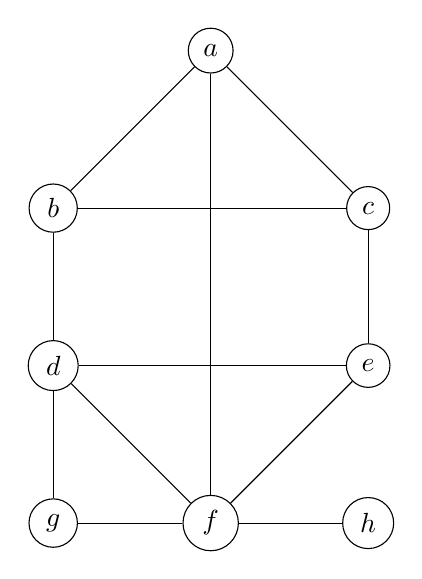
\begin{tikzpicture}
    \node (a) [draw,circle] at (2,6) {\(a\)};
    \node (b) [draw,circle] at (0,4) {\(b\)};
    \node (c) [draw,circle] at (4,4) {\(c\)};
    \node (d) [draw,circle] at (0,2) {\(d\)};
    \node (e) [draw,circle] at (4,2) {\(e\)};
    \node (f) [draw,circle] at (2,0) {\(f\)};
    \node (g) [draw,circle] at (0,0) {\(g\)};
    \node (h) [draw,circle] at (4,0) {\(h\)};
    \draw (a) to (b);
    \draw (a) to (c);
    \draw (a) to (f);
    \draw (b) to (c);
    \draw (b) to (d);
    \draw (c) to (e);
    \draw (d) to (e);
    \draw (d) to (f);
    \draw (d) to (g);
    \draw (e) to (f);
    \draw (f) to (g);
    \draw (f) to (h);
  \end{tikzpicture}
  \caption{An example graph.}
  \label{fig:example}
\end{figure}

The algorithm steps are as follows.  Main routine steps are marked by ``O\#'' and recursive subroutine steps are
marked by ``I\#.''.  Recursive subroutine calls add a call level: ``I\#--\#.''

\begin{enumerate}
\item (O\ref{step:outer:bron}) Use the Bron Kerbosch algorithm to calculate \(k_{min}=3\).

\item (O\ref{step:outer:greedy}) Use the greedy last-first algorithm to calculate \(k_{max}=4\).

\item (O\ref{step:outer:initk}) Initialize \(k=k_{min}=3\).

\item (O\ref{step:outer:match}) \(k=3\ne4=k_{max}\), so continue.

\item (O\ref{step:outer:call}) Call the subroutine with \(G\) and \(k=3\).

\item (I\ref{step:sub:check}) \(n=8\nleq3=k\), so continue.

\item (I\ref{step:sub:dencalc}) Calculate the maximum edge threshold for \(n=8\) and \(k=3\):
  \[a=\frac{n^2(k-1)}{2k}=\frac{8^2(3-1)}{2\cdot3}\approx21.3\]

\item (I\ref{step:sub:density}) \(m=12\ngtr21.3=a\), so continue.

\item (I\ref{step:sub:smallcalc}) \(\deg(g)=2<3\) and \(\deg(h)=1<3\), so set \(X=\set{g,h}\).

\item (I\ref{step:sub:small}) \(X\ne\emptyset\), so replace \(G\) with \(G-X\).  The result is shown in
  \figurename~\ref{fig:removegh}.  Now \(n=6\) and \(m=9\).

  \begin{figure}[H]
    \centering
    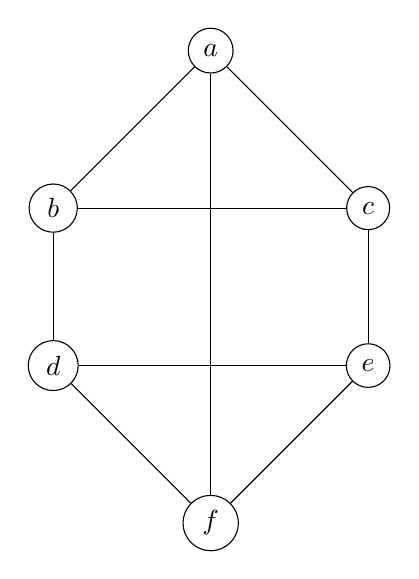
\begin{tikzpicture}
      \node (a) [draw,circle] at (2,6) {\(a\)};
      \node (b) [draw,circle] at (0,4) {\(b\)};
      \node (c) [draw,circle] at (4,4) {\(c\)};
      \node (d) [draw,circle] at (0,2) {\(d\)};
      \node (e) [draw,circle] at (4,2) {\(e\)};
      \node (f) [draw,circle] at (2,0) {\(f\)};
      \draw (a) to (b);
      \draw (a) to (c);
      \draw (a) to (f);
      \draw (b) to (c);
      \draw (b) to (d);
      \draw (c) to (e);
      \draw (d) to (e);
      \draw (d) to (f);
      \draw (e) to (f);
    \end{tikzpicture}
    \caption{Step: \(G-\set{g,h}\).}
    \label{fig:removegh}
  \end{figure}

\item (I\ref{step:sub:check}) \(n=6\nleq3=k\), so continue.

\item (I\ref{step:sub:dencalc}) Calculate the maximum edge threshold for \(n=6\) and \(k=3\):
  \[a=\frac{n^2(k-1)}{2k}=\frac{6^2(3-1)}{2\cdot3}=12\]

\item (I\ref{step:sub:density}) \(m=12\ngtr12=a\), so continue.

\item (I\ref{step:sub:smallcalc}) \(\dmin(G)=3\ge3=k\), so set \(X=\emptyset\).

\item (I\ref{step:sub:small}) \(X=\emptyset\), so continue.

\item (I\ref{step:sub:common}) Calculate the number of common neighbors, looking for any subsets.  The results are
  shown in \tablename~\ref{tab:common}.

  \begin{table}[H]
    \centering
    \caption{Calculating Common Neighbors}
    \label{tab:common}
    \begin{tabular}{|c|c|c|c|c|}
      \hline
      \(u\) & \(v\) & \(\abs{N(u)\cap N(v)}\) & subset? & adjacent? \\
      \hline
      \(a\) & \(b\) & 1 & N & Y \\
      \hline
      \(a\) & \(c\) & 1 & N & Y \\
      \hline
      \(a\) & \(d\) & 2 & N & N \\
      \hline
      \(a\) & \(e\) & 2 & N & N \\
      \hline
      \(a\) & \(f\) & 0 & N & Y \\
      \hline
      \(b\) & \(c\) & 1 & N & Y \\
      \hline
      \(b\) & \(d\) & 0 & N & Y \\
      \hline
      \(b\) & \(e\) & 2 & N & N \\
      \hline
      \(b\) & \(f\) & 2 & N & N \\
      \hline
      \(c\) & \(d\) & 2 & N & N \\
      \hline
      \(c\) & \(e\) & 0 & N & Y \\
      \hline
      \(c\) & \(f\) & 2 & N & N \\
      \hline
      \(d\) & \(e\) & 1 & N & Y \\
      \hline
      \(d\) & \(f\) & 1 & N & Y \\
      \hline
      \(e\) & \(f\) & 1 & N & Y \\
      \hline
    \end{tabular}
  \end{table}

\item (I\ref{step:sub:subset}) There are no \(u,v\in V(G)\) such that \(N(u)\subseteq N(v)\), so continue.

\item (I\ref{step:sub:select}) From \tablename~\ref{tab:common}, the minimum number of common neighbors is 0
  (e.g., \(a\) and \(f\)), so set \(b=0\).

\item (I\ref{step:sub:ubcalc}) Calculate the upper bound for minimum number of common neighbors for \(n=6\) and
  \(k=3\):
  \[c=n-2-\frac{n-2}{k-1}=6-2-\frac{6-2}{3-1}=2\]

\item (I\ref{step:sub:ubcheck}) \(b=0\ngtr2=c\), so conclude that \(G\) may be \colorable{3} and continue.

\item (I\ref{step:sub:select2}) Based on the results in \tablename~\ref{tab:common}, all of the nonadjacent
  vertices share two common neighbors, so select \(a\) and \(d\).

\item (I\ref{step:sub:call1}) Recursively call the subroutine with \(G\cdot ad\), as shown in
  \figurename~\ref{fig:contractad}.  Now, \(n=5\) and \(m=7\).

  \begin{figure}[H]
    \centering
    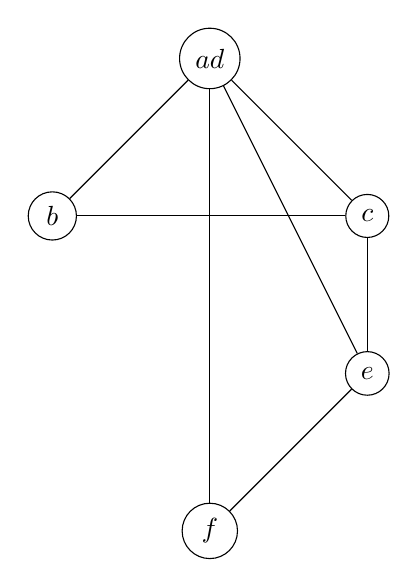
\begin{tikzpicture}
      \node (ad) [draw,circle] at (2,6) {\(ad\)};
      \node (b) [draw,circle] at (0,4) {\(b\)};
      \node (c) [draw,circle] at (4,4) {\(c\)};
      \node (e) [draw,circle] at (4,2) {\(e\)};
      \node (f) [draw,circle] at (2,0) {\(f\)};
      \draw (ad) to (b);
      \draw (ad) to (c);
      \draw (ad) to (f);
      \draw (b) to (c);
      \draw (c) to (e);
      \draw (ad) to (e);
      \draw (e) to (f);
    \end{tikzpicture}
    \caption{Step: \(G\cdot ad\).}
    \label{fig:contractad}
  \end{figure}

\item (I\ref{step:sub:check}-1) \(n=5\nleq3=k\), so continue.

\item (I\ref{step:sub:dencalc}-1) Calculate the maximum edge threshold for \(n=5\) and \(k=3\):
  \[a=\frac{n^2(k-1)}{2k}=\frac{5^2(3-1)}{2\cdot3}\approx8.3\]

\item (I\ref{step:sub:density}-1) \(m=7\ngtr8.3=a\), so conclude that \(G\) may be \colorable{3} and continue.
  
\item (I\ref{step:sub:smallcalc}-1) \(\deg(b)=\deg(f)=2<3=k\), so set \(X=\set{b,f}\).

\item (I1-\ref{step:sub:small}-1) \(X\ne\emptyset\), so replace \(G\) with \(G-X\).  The result is shown in Figure
  \ref{fig:removecf}.  Now \(n=3\) and \(m=3\).

  \begin{figure}[H]
    \centering
    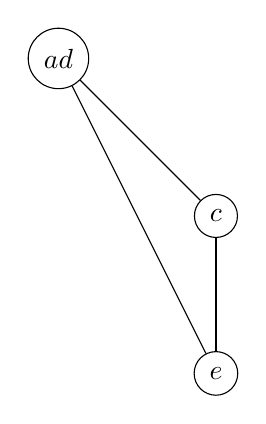
\begin{tikzpicture}
      \node (ad) [draw,circle] at (2,6) {\(ad\)};
      \node (c) [draw,circle] at (4,4) {\(c\)};
      \node (e) [draw,circle] at (4,2) {\(e\)};
      \draw (ad) to (c);
      \draw (c) to (e);
      \draw (e) to (ad);
    \end{tikzpicture}
    \caption{Step: \(G-\set{b,f}\)}
    \label{fig:removecf}
  \end{figure}

\item (I\ref{step:sub:check}-1) \(n=3\le3=k\), so conclude that the \(G\) of \figurename~\ref{fig:removecf} is
  \colorable{3} and return true.

\item (I\ref{step:sub:result1}) The recursive call returned true, so conclude that the \(G\) of
  \figurename~\ref{fig:removecf} is \colorable{3} and return true.

\item (O\ref{step:outer:result})\label{step:last} The recursive subroutine returned true, so conclude that the \(G\)
  is \chromatic{3} and return \(\X(G)=3\).
\end{enumerate}

Thus, the algorithm determines that the example \(G\) of Figure \ref{fig:example} is \chromatic{3} in
\ref{step:last} steps.  In order to determine a \chromatic{3} coloring for \(G\), first construct a set \(C\) of
three colors:
\[C=\set{\text{\textcolor{green}{green}},\text{\textcolor{blue}{blue}},\text{\textcolor{red}{red}}}\]
Next, follow the algorithm's modification steps in reverse order and color the corresponding vertices accordingly.
The steps are as follows:

\begin{enumerate}
\item First, color the vertices that are present in the final simplified graph.  Assign each vertex its own color,
  except assign contracted vertices the same color.  This is shown in \figurename~\ref{fig:cstart}.
  
  \begin{figure}[H]
    \centering
    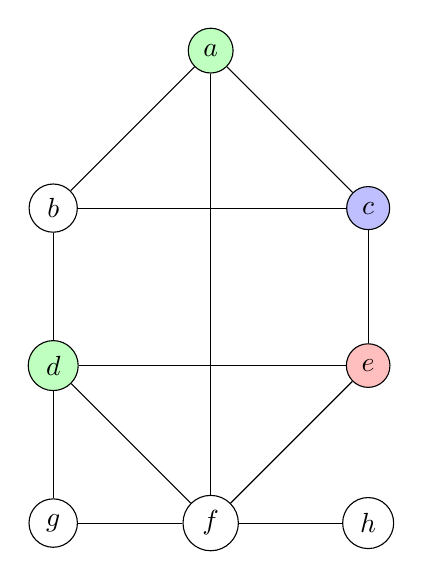
\begin{tikzpicture}
      \colorlet{c1}{green!25!white}
      \colorlet{c2}{blue!25!white}
      \colorlet{c3}{red!25!white}
      \node [fill=c1] (a) [draw,circle] at (2,6) {\(a\)};
      \node (b) [draw,circle] at (0,4) {\(b\)};
      \node [fill=c2] (c) [draw,circle] at (4,4) {\(c\)};
      \node [fill=c1] (d) [draw,circle] at (0,2) {\(d\)};
      \node [fill=c3] (e) [draw,circle] at (4,2) {\(e\)};
      \node (f) [draw,circle] at (2,0) {\(f\)};
      \node (g) [draw,circle] at (0,0) {\(g\)};
      \node (h) [draw,circle] at (4,0) {\(h\)};
      \draw (a) to (b);
      \draw (a) to (c);
      \draw (a) to (f);
      \draw (b) to (c);
      \draw (b) to (d);
      \draw (c) to (e);
      \draw (d) to (e);
      \draw (d) to (f);
      \draw (d) to (g);
      \draw (e) to (f);
      \draw (f) to (g);
      \draw (f) to (h);
    \end{tikzpicture}
    \caption{Initial coloring.}
    \label{fig:cstart}
  \end{figure}

\item The last modification was the removal of vertices \(b\) and \(f\).  Note that color selection needs to honor
  the vertices already colored.  This is shown in \figurename~\ref{fig:colorbf}.

  \begin{figure}[H]
    \centering
    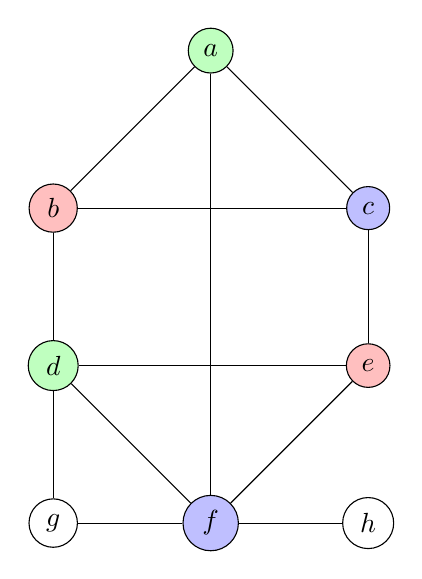
\begin{tikzpicture}
      \colorlet{c1}{green!25!white}
      \colorlet{c2}{blue!25!white}
      \colorlet{c3}{red!25!white}
      \node [fill=c1] (a) [draw,circle] at (2,6) {\(a\)};
      \node [fill=c3] (b) [draw,circle] at (0,4) {\(b\)};
      \node [fill=c2] (c) [draw,circle] at (4,4) {\(c\)};
      \node [fill=c1] (d) [draw,circle] at (0,2) {\(d\)};
      \node [fill=c3] (e) [draw,circle] at (4,2) {\(e\)};
      \node [fill=c2] (f) [draw,circle] at (2,0) {\(f\)};
      \node (g) [draw,circle] at (0,0) {\(g\)};
      \node (h) [draw,circle] at (4,0) {\(h\)};
      \draw (a) to (b);
      \draw (a) to (c);
      \draw (a) to (f);
      \draw (b) to (c);
      \draw (b) to (d);
      \draw (c) to (e);
      \draw (d) to (e);
      \draw (d) to (f);
      \draw (d) to (g);
      \draw (e) to (f);
      \draw (f) to (g);
      \draw (f) to (h);
    \end{tikzpicture}
    \caption{Coloring \(b\) and \(f\).}
    \label{fig:colorbf}
  \end{figure}

\item Finally, color the first removed vertices \(g\) and \(h\) with any appropriate color.  The final result is
  shown in \figurename~\ref{fig:cfinal}.

  \begin{figure}[H]
    \centering
    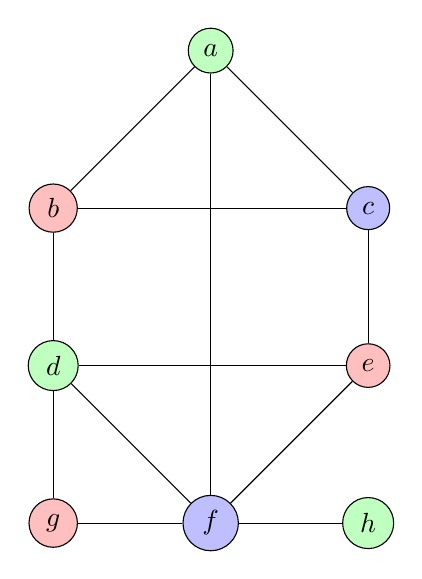
\begin{tikzpicture}
      \colorlet{c1}{green!25!white}
      \colorlet{c2}{blue!25!white}
      \colorlet{c3}{red!25!white}
      \node [fill=c1] (a) [draw,circle] at (2,6) {\(a\)};
      \node [fill=c3] (b) [draw,circle] at (0,4) {\(b\)};
      \node [fill=c2] (c) [draw,circle] at (4,4) {\(c\)};
      \node [fill=c1] (d) [draw,circle] at (0,2) {\(d\)};
      \node [fill=c3] (e) [draw,circle] at (4,2) {\(e\)};
      \node [fill=c2] (f) [draw,circle] at (2,0) {\(f\)};
      \node [fill=c3] (g) [draw,circle] at (0,0) {\(g\)};
      \node [fill=c1] (h) [draw,circle] at (4,0) {\(h\)};
      \draw (a) to (b);
      \draw (a) to (c);
      \draw (a) to (f);
      \draw (b) to (c);
      \draw (b) to (d);
      \draw (c) to (e);
      \draw (d) to (e);
      \draw (d) to (f);
      \draw (d) to (g);
      \draw (e) to (f);
      \draw (f) to (g);
      \draw (f) to (h);
    \end{tikzpicture}
    \caption{Final chromatic coloring.}
    \label{fig:cfinal}
  \end{figure}

\end{enumerate}

At first glance, one might wonder what advantage this method of coloring has over other sequential methods.  The
difference is that the other sequential methods only have knowledge about what has already been colored, whereas
this method uses assumptions that are made during the simplifications and recursive calls on the entire graph.
Thus, the sequential algorithms are heuristic, but this method selects a particular workable coloring path through
the resulting Zykov tree.

\section{An Example}

In this section, the proposed algorithm will be applied to the example graph \(G\) (\(n=8\) and \(m=12\)) shown in
Figure \ref{fig:example} in order to determine its chromatic number.  The steps of the algorithm are then traversed
in reverse order to determine a chromatic coloring.

\begin{figure}[h]
  \label{fig:example}
  \begin{center}
    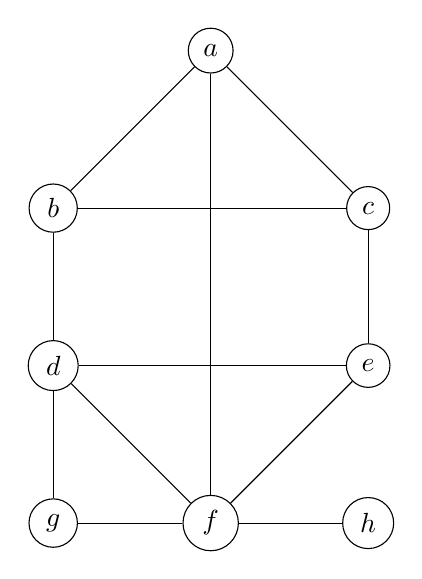
\begin{tikzpicture}
      \node (a) [draw,circle] at (2,6) {\(a\)};
      \node (b) [draw,circle] at (0,4) {\(b\)};
      \node (c) [draw,circle] at (4,4) {\(c\)};
      \node (d) [draw,circle] at (0,2) {\(d\)};
      \node (e) [draw,circle] at (4,2) {\(e\)};
      \node (f) [draw,circle] at (2,0) {\(f\)};
      \node (g) [draw,circle] at (0,0) {\(g\)};
      \node (h) [draw,circle] at (4,0) {\(h\)};
      \draw (a) to (b);
      \draw (a) to (c);
      \draw (a) to (f);
      \draw (b) to (c);
      \draw (b) to (d);
      \draw (c) to (e);
      \draw (d) to (e);
      \draw (d) to (f);
      \draw (d) to (g);
      \draw (e) to (f);
      \draw (f) to (g);
      \draw (f) to (h);
    \end{tikzpicture}
  \end{center}
  \caption{Example Graph}
\end{figure}

The algorithm steps are as follows.  Outer loop steps are marked by ``O\#'' and called subroutine steps are marked by
``I\#.''.  Recursive subroutine calls add a call level: ``I\#--\#.''

\begin{enumerate}
\item (O\ref{step:null}) Since \(n=8>0\), \(G\) is not the null graph, so continue.

\item (O\ref{step:one}) Since \(n=8>1\), \(G\) is not an empty graph, so continue.

\item (O\ref{step:init}) Initialize \(k\) to 2.

\item (O\ref{step:inner}) Call the subroutine with \(G\) and \(k=2\).

\item (I\ref{step:check}) \(n=8\nleq k=2\), so continue.

\item (I\ref{step:dencalc}) Calculate the maximum edge threshold for \(n=8\) and \(k=2\):
  \[a=\frac{n^2(k-1)}{2k}=\frac{8^2(2-1)}{2\cdot2}=\frac{64}{4}=16\]

\item (I\ref{step:density}) Since \(m=12\ngtr16=a\), continue.

\item (I\ref{step:smallcalc}) Since \(\deg(h)=1<2\), set \(X=\set{h}\).

\item (I\ref{step:small}) Since \(X\ne\emptyset\), replace \(G\) with \(G-X\).  The result is shown in Figure
  \ref{fig:removeh}.  Now \(n=7\) and \(m=11\).

  \begin{figure}[h]
    \label{fig:removeh}
    \begin{center}
      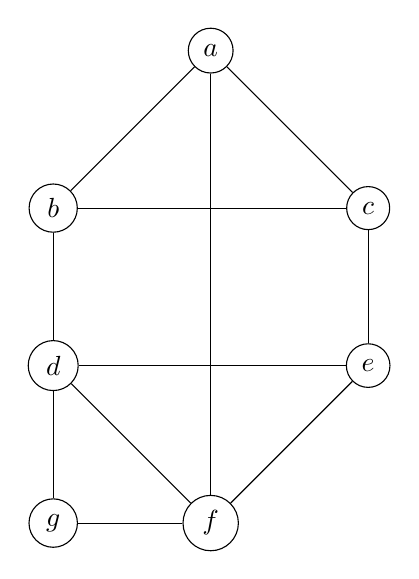
\begin{tikzpicture}
        \node (a) [draw,circle] at (2,6) {\(a\)};
        \node (b) [draw,circle] at (0,4) {\(b\)};
        \node (c) [draw,circle] at (4,4) {\(c\)};
        \node (d) [draw,circle] at (0,2) {\(d\)};
        \node (e) [draw,circle] at (4,2) {\(e\)};
        \node (f) [draw,circle] at (2,0) {\(f\)};
        \node (g) [draw,circle] at (0,0) {\(g\)};
        \draw (a) to (b);
        \draw (a) to (c);
        \draw (a) to (f);
        \draw (b) to (c);
        \draw (b) to (d);
        \draw (c) to (e);
        \draw (d) to (e);
        \draw (d) to (f);
        \draw (d) to (g);
        \draw (e) to (f);
        \draw (f) to (g);
      \end{tikzpicture}
    \end{center}
    \caption{\(G-\set{h}\)}
  \end{figure}

\item (I\ref{step:check}) \(n=7\nleq k=2\), so continue.

\item (I\ref{step:dencalc}) Calculate the maximum edge threshold for \(n=7\) and \(k=2\):
  \[a=\frac{n^2(k-1)}{2k}=\frac{7^2(2-1)}{2\cdot2}=\frac{49}{4}\approx12.3\]

\item (I\ref{step:density}) Since \(m=12\ngtr12.3=a\), continue.

\item (I\ref{step:smallcalc}) Since \(\d(G)=2\ge2=k\), set \(X=\emptyset\).

\item (I\ref{step:small}) Since \(X=\emptyset\), continue.

\item (I\ref{step:neighbor}) Note that \(N(g)=\set{d,f}\) and \(N(e)=\set{c,d,f}\).  Since \(N(g)\subseteq N(e)\),
  replace \(G\) with \(G-g\).  The result is shown in Figure \ref{fig:removeg}.  Now \(n=6\) and \(m=9\).

  \begin{figure}[h]
    \label{fig:removeg}
    \begin{center}
      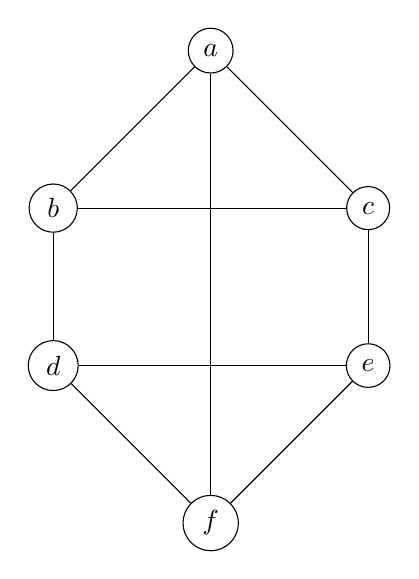
\begin{tikzpicture}
        \node (a) [draw,circle] at (2,6) {\(a\)};
        \node (b) [draw,circle] at (0,4) {\(b\)};
        \node (c) [draw,circle] at (4,4) {\(c\)};
        \node (d) [draw,circle] at (0,2) {\(d\)};
        \node (e) [draw,circle] at (4,2) {\(e\)};
        \node (f) [draw,circle] at (2,0) {\(f\)};
        \draw (a) to (b);
        \draw (a) to (c);
        \draw (a) to (f);
        \draw (b) to (c);
        \draw (b) to (d);
        \draw (c) to (e);
        \draw (d) to (e);
        \draw (d) to (f);
        \draw (e) to (f);
      \end{tikzpicture}
    \end{center}
    \caption{\(G-g\)}
  \end{figure}

\item (I\ref{step:check}) \(n=6\nleq k=2\), so continue.

\item (I\ref{step:dencalc}) Calculate the maximum edge threshold for \(n=6\) and \(k=2\):
  \[a=\frac{n^2(k-1)}{2k}=\frac{6^2(2-1)}{2\cdot2}=\frac{36}{4}=9\]

\item (I\ref{step:density}) Since \(m=9\ngtr9=a\), continue.

\item (I\ref{step:smallcalc}) Since \(\d(G)=2\ge2=k\), set \(X=\emptyset\).

\item (I\ref{step:small}) Since \(X=\emptyset\), continue.

\item (I\ref{step:neighbor}) Since there is no \(N(u)\subseteq N(v)\), continue.

\item (I\ref{step:select}) Note that due to the symmetry of \(G\) every two vertices share exactly two neighbors:
  \[b=\min_{u,v\in V(G)}\abs{N(u)\cap N(v)]}=2\]

\item (I\ref{step:neighcalc}) Calculate the upper bound for minimum number of common neighbors for \(n=6\) and
  \(k=2\):
  \[c=n-2-\frac{n-2}{k-1}=6-2-\frac{6-2}{2-1}=4-4=0\]

\item (I\ref{step:common}) Since \(b=2>0=c\), conclude that \(G\) is not \colorable{2}.  Return false and the current
  state of \(G\) to the outer loop.

\item (O\ref{step:call}) Since the called subroutine returned false, \(G\) is not \colorable{2}, so continue.

\item (O\ref{step:newg}) Replace \(G\) with the graph returned by the previous call (Figure \ref{fig:removeg}).

\item (O\ref{step:incr}) Increment \(k\) to 3.

\item (O\ref{step:inner}) Call the subroutine with the new \(G\) and \(k=3\).
  
\item (I\ref{step:check}) \(n=6\nleq k=3\), so continue.

\item (I\ref{step:dencalc}) Calculate the maximum edge threshold for \(n=6\) and \(k=3\):
  \[a=\frac{n^2(k-1)}{2k}=\frac{6^2(3-1)}{2\cdot3}=\frac{72}{6}=12\]

\item (I\ref{step:density}) Since \(m=9\ngtr11=a\), continue.

\item (I\ref{step:smallcalc}) Since \(\d(G)=3\ge3=k\), set \(X=\emptyset\).

\item (I\ref{step:small}) Since \(X=\emptyset\), continue.

\item (I\ref{step:select}) Note that due to the symmetry of \(G\) every two vertices share exactly two neighbors:
  \[b=\min_{u,v\in V(G)}\abs{N(u)\cap N(v)]}=2\]

\item (I\ref{step:neighcalc}) Calculate the upper bound for minimum number of common neighbors for \(n=6\) and
  \(k=3\):
  \[c=n-2-\frac{n-2}{k-1}=6-2-\frac{6-2}{3-1}=4-2=2\]

\item (I\ref{step:common}) Since \(b=2\ngtr2=c\), continue.

\item (I\ref{step:select2}) Since every two vertices share exactly two neighbors, select any two non-adjacent
  vertices: \(a\) and \(e\).

\item (I\ref{step:call1}) Recursively call the subroutine with \(G\cdot ae\) and \(k=3\).  The result is shown in
  Figure \ref{fig:conae}.  Now \(n=5\) and \(m=7\).

  \begin{figure}[h]
    \label{fig:conae}
    \begin{center}
      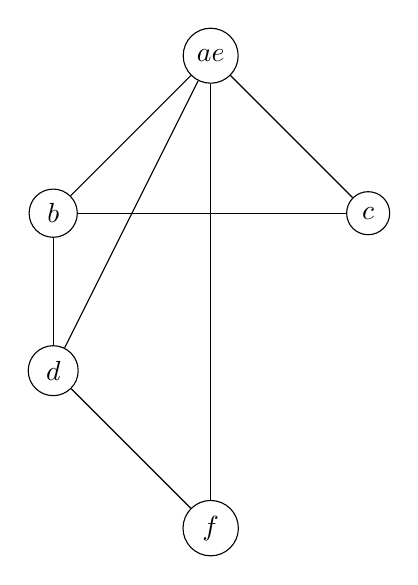
\begin{tikzpicture}
        \node (ae) [draw,circle] at (2,6) {\(ae\)};
        \node (b) [draw,circle] at (0,4) {\(b\)};
        \node (c) [draw,circle] at (4,4) {\(c\)};
        \node (d) [draw,circle] at (0,2) {\(d\)};
        \node (f) [draw,circle] at (2,0) {\(f\)};
        \draw (ae) to (b);
        \draw (ae) to (c);
        \draw (ae) to (f);
        \draw (b) to (c);
        \draw (b) to (d);
        \draw (d) to (ae);
        \draw (d) to (f);
      \end{tikzpicture}
    \end{center}
    \caption{\(G\cdot ae\)}
  \end{figure}

\item (I1-\ref{step:check}) \(n=5\nleq k=3\), so continue.

\item (I1-\ref{step:dencalc}) Calculate the maximum edge threshold for \(n=5\) and \(k=3\):
  \[a=\frac{n^2(k-1)}{2k}=\frac{5^2(3-1)}{2\cdot3}=\frac{50}{6}\approx8.3\]

\item (I1-\ref{step:density}) Since \(m=7\ngtr8.3=a\), continue.

\item (I1-\ref{step:smallcalc}) Since \(\deg(c)=\deg(f)=2<3=k\), set \(X=\set{c,f}\).

\item (I1-\ref{step:small}) Since \(X\ne\emptyset\), replace \(G\) with \(G-X\).  The result is shown in Figure
  \ref{fig:removecf}.  Now \(n=3\) and \(m=3\).

  \begin{figure}[h]
    \label{fig:removecf}
    \begin{center}
      \begin{tikzpicture}
        \node (ae) [draw,circle] at (2,6) {\(ae\)};
        \node (b) [draw,circle] at (0,4) {\(b\)};
        \node (d) [draw,circle] at (0,2) {\(d\)};
        \draw (ae) to (b);
        \draw (b) to (d);
        \draw (d) to (a);
      \end{tikzpicture}
    \end{center}
    \caption{\(G-\set{c,f}\)}
  \end{figure}

\item (I1-\ref{step:check}) \(n=3\le k=3\), so conclude that \(G\) is \colorable{3} and return true.

\item (I\ref{step:call1}) The recursive call returned true, so conclude that \(G\) is \colorable{3} and return true.

\item (O\ref{step:call}) The called subroutine returned true, so conclude that \(G\) is \chromatic{3} and return
  \(\X(G)=3\).

\end{enumerate}

So the algorithm determines that the example \(G\) of Figure \ref{fig:example} is \chromatic{3}.  In order to
determine a \chromatic{3} coloring for \(G\), first construct a set \(C\) of three colors:
\[C=\set{\text{\textcolor{green}{green}},\text{\textcolor{blue}{blue}},\text{\textcolor{red}{red}}}\]
Next, follow the algorithm's modification steps in reverse order and color the corresponding vertices accordingly.
The steps are as follows:

\begin{enumerate}
\item First, color the vertices that are present in the final simplified graph.  Assign each vertex its own color,
  except assign contracted vertices the same color.  This is shown in Figure \ref{fig:cstart}.
  
  \begin{figure}[h]
    \label{fig:cstart}
    \begin{center}
      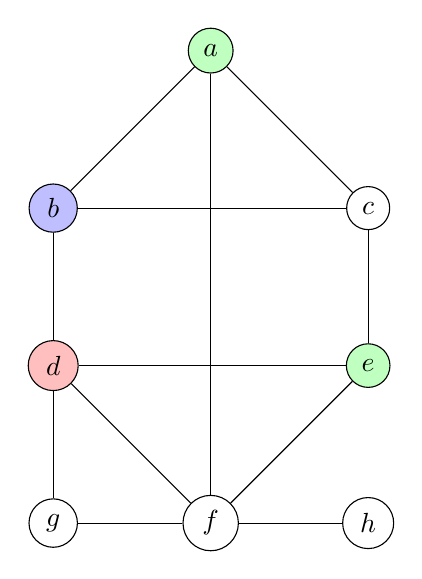
\begin{tikzpicture}
        \colorlet{c1}{green!25!white}
        \colorlet{c2}{blue!25!white}
        \colorlet{c3}{red!25!white}
        \node [fill=c1] (a) [draw,circle] at (2,6) {\(a\)};
        \node [fill=c2] (b) [draw,circle] at (0,4) {\(b\)};
        \node (c) [draw,circle] at (4,4) {\(c\)};
        \node [fill=c3] (d) [draw,circle] at (0,2) {\(d\)};
        \node [fill=c1] (e) [draw,circle] at (4,2) {\(e\)};
        \node (f) [draw,circle] at (2,0) {\(f\)};
        \node (g) [draw,circle] at (0,0) {\(g\)};
        \node (h) [draw,circle] at (4,0) {\(h\)};
        \draw (a) to (b);
        \draw (a) to (c);
        \draw (a) to (f);
        \draw (b) to (c);
        \draw (b) to (d);
        \draw (c) to (e);
        \draw (d) to (e);
        \draw (d) to (f);
        \draw (d) to (g);
        \draw (e) to (f);
        \draw (f) to (g);
        \draw (f) to (h);
      \end{tikzpicture}
    \end{center}
    \caption{Initial Coloring}
  \end{figure}

\item The last modification was the removal of vertices \(c\) and \(f\).  Note that color selection needs to honor
  the vertices already colored.  This is shown in Figure \ref{fig:colorcf}.

  \begin{figure}[h]
    \label{fig:colorcf}
    \begin{center}
      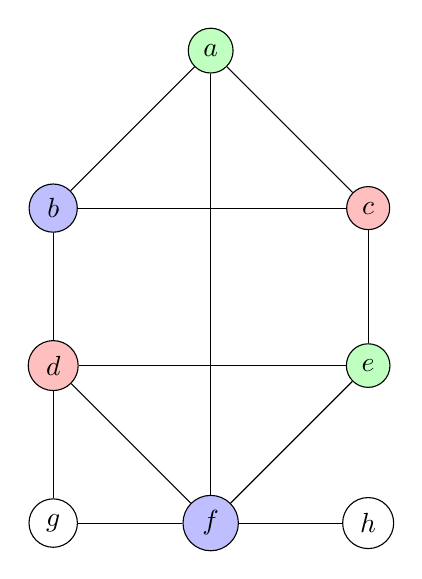
\begin{tikzpicture}
        \colorlet{c1}{green!25!white}
        \colorlet{c2}{blue!25!white}
        \colorlet{c3}{red!25!white}
        \node [fill=c1] (a) [draw,circle] at (2,6) {\(a\)};
        \node [fill=c2] (b) [draw,circle] at (0,4) {\(b\)};
        \node [fill=c3] (c) [draw,circle] at (4,4) {\(c\)};
        \node [fill=c3] (d) [draw,circle] at (0,2) {\(d\)};
        \node [fill=c1] (e) [draw,circle] at (4,2) {\(e\)};
        \node [fill=c2] (f) [draw,circle] at (2,0) {\(f\)};
        \node (g) [draw,circle] at (0,0) {\(g\)};
        \node (h) [draw,circle] at (4,0) {\(h\)};
        \draw (a) to (b);
        \draw (a) to (c);
        \draw (a) to (f);
        \draw (b) to (c);
        \draw (b) to (d);
        \draw (c) to (e);
        \draw (d) to (e);
        \draw (d) to (f);
        \draw (d) to (g);
        \draw (e) to (f);
        \draw (f) to (g);
        \draw (f) to (h);
      \end{tikzpicture}
    \end{center}
    \caption{Coloring \(c\) and \(f\)}
  \end{figure}

\item The contracted vertices have already been colored, so the next simplification to address is the removal of
  \(g\) due to the neighborhood subset test.  Since \(N(g)\subseteq N(e)\), color \(g\) and \(e\) the same color.
  Since \(e\) has already been assign a color, use it for \(g\).  The result is shown in Figure \ref{fig:colorg}.

  \begin{figure}[h]
    \label{fig:colorg}
    \begin{center}
      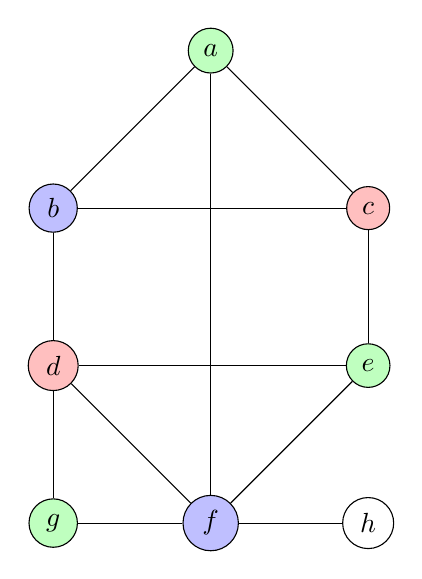
\begin{tikzpicture}
        \colorlet{c1}{green!25!white}
        \colorlet{c2}{blue!25!white}
        \colorlet{c3}{red!25!white}
        \node [fill=c1] (a) [draw,circle] at (2,6) {\(a\)};
        \node [fill=c2] (b) [draw,circle] at (0,4) {\(b\)};
        \node [fill=c3] (c) [draw,circle] at (4,4) {\(c\)};
        \node [fill=c3] (d) [draw,circle] at (0,2) {\(d\)};
        \node [fill=c1] (e) [draw,circle] at (4,2) {\(e\)};
        \node [fill=c2] (f) [draw,circle] at (2,0) {\(f\)};
        \node [fill=c1] (g) [draw,circle] at (0,0) {\(g\)};
        \node (h) [draw,circle] at (4,0) {\(h\)};
        \draw (a) to (b);
        \draw (a) to (c);
        \draw (a) to (f);
        \draw (b) to (c);
        \draw (b) to (d);
        \draw (c) to (e);
        \draw (d) to (e);
        \draw (d) to (f);
        \draw (d) to (g);
        \draw (e) to (f);
        \draw (f) to (g);
        \draw (f) to (h);
      \end{tikzpicture}
    \end{center}
    \caption{Coloring \(g\)}
  \end{figure}

\item Finally, color the first removed vertex \(h\) with any appropriate color.  The final result is shown in
  Figure \ref{fig:cfinal}.

  \begin{figure}[h]
    \label{fig:cfinal}
    \begin{center}
      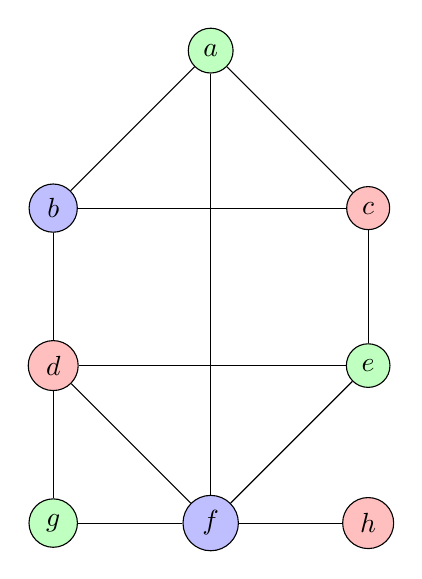
\begin{tikzpicture}
        \colorlet{c1}{green!25!white}
        \colorlet{c2}{blue!25!white}
        \colorlet{c3}{red!25!white}
        \node [fill=c1] (a) [draw,circle] at (2,6) {\(a\)};
        \node [fill=c2] (b) [draw,circle] at (0,4) {\(b\)};
        \node [fill=c3] (c) [draw,circle] at (4,4) {\(c\)};
        \node [fill=c3] (d) [draw,circle] at (0,2) {\(d\)};
        \node [fill=c1] (e) [draw,circle] at (4,2) {\(e\)};
        \node [fill=c2] (f) [draw,circle] at (2,0) {\(f\)};
        \node [fill=c1] (g) [draw,circle] at (0,0) {\(g\)};
        \node [fill=c3] (h) [draw,circle] at (4,0) {\(h\)};
        \draw (a) to (b);
        \draw (a) to (c);
        \draw (a) to (f);
        \draw (b) to (c);
        \draw (b) to (d);
        \draw (c) to (e);
        \draw (d) to (e);
        \draw (d) to (f);
        \draw (d) to (g);
        \draw (e) to (f);
        \draw (f) to (g);
        \draw (f) to (h);
      \end{tikzpicture}
    \end{center}
    \caption{Final Chromatic Coloring}
  \end{figure}

\end{enumerate}

At first glance, one might wonder what advantage this method of coloring has over greedy coloring.  The difference
is that greedy coloring only has knowledge about what has already been colored, whereas this method uses
assumptions that are made during the simplifications and recursive calls on the entire graph.  Thus, the greedy
algorithm is heuristic, but this method selects a particular workable coloring path through the modified Zykov
tree.  In this way, this method is not so much different from the exhaustive algorithm.

\section{Toaster Design Case Study}

This section contains a simplistic case study of how the proposed algorithm could be used to compare the functional
requirement (FR) graphs resulting from two slightly different designs of the basic kitchen toaster shown in
Figure \ref{fig:toaster}.

\begin{figure}[h]
  \label{fig:toaster}
  \begin{center}
    \includegraphics[scale=0.2]{toaster}
  \end{center}
  \caption{Example Toaster}
\end{figure}

The functional requirements (FRs) are shown in Table \ref{toasterfrs}.  It is assumed that the design is either
uncoupled or decoupled and hence the independence of the FRs is as strong as possible.

\begin{table}[h]
  \label{toasterfrs}
  \begin{center}
    \begin{tabular}{|c|l|}
      \hline
      FR1 & Body contains all parts \\
      \hline
      FR2 & Can be safely moved while hot \\
      \hline
      FR3 & Can hold two slices of bread \\
      \hline
      FR4 & Heats each slice of bread on both sides \\
      \hline
      FR5 & Toasting is manually started \\
      \hline
      FR6 & Toasting is automatically or can be manually stopped \\
      \hline
      FR7 & Heat level can be controlled \\
      \hline
    \end{tabular}
  \end{center}
  \caption{Toaster Functional Requirements}
\end{table}

The graph \(G_1\) for the first candidate design with \(n=7\) and \(m=13\) is shown in Figure \ref{fig:design1}.

\begin{figure}[h]
  \label{fig:design1}
  \begin{center}
    \scalebox{0.75}{
      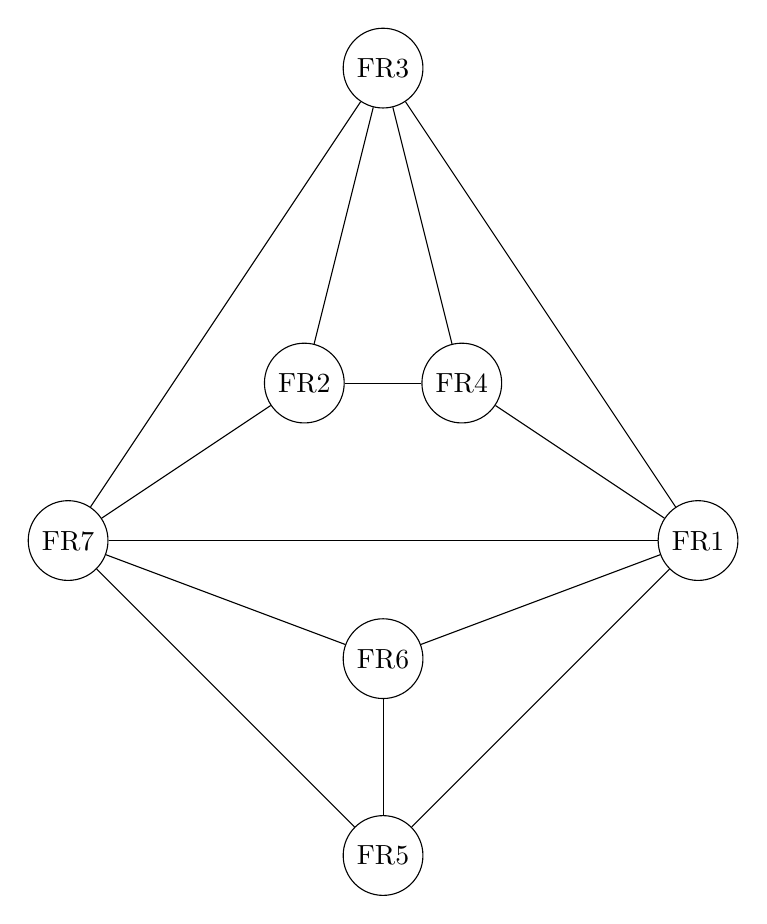
\begin{tikzpicture}
        \node [draw,circle] (fr1) at (4,0) {FR1};
        \node [draw,circle] (fr2) at (-1,2) {FR2};
        \node [draw,circle] (fr3) at (0,6) {FR3};
        \node [draw,circle] (fr4) at (1,2) {FR4};
        \node [draw,circle] (fr5) at (0,-4) {FR5};
        \node [draw,circle] (fr6) at (0,-1.5) {FR6};
        \node [draw,circle] (fr7) at (-4,0) {FR7};
        \draw (fr1) edge (fr3);
        \draw (fr1) edge (fr4);
        \draw (fr1) edge (fr5);
        \draw (fr1) edge (fr6);
        \draw (fr1) edge (fr7);
        \draw (fr2) edge (fr3);
        \draw (fr2) edge (fr4);
        \draw (fr2) edge (fr7);
        \draw (fr3) edge (fr4);
        \draw (fr3) edge (fr7);
        \draw (fr5) edge (fr6);
        \draw (fr5) edge (fr7);
        \draw (fr6) edge (fr7);
      \end{tikzpicture}
    }

    \bigskip

    \(G_1\)
  \end{center}
  \caption{First Candidate Design}
\end{figure}

For \(k=2\), the maximum edge threshold test fails:
\[\frac{n^2(k-1)}{2k}=\frac{7^2(2-1)}{2\cdot2}=\frac{49}{4}\approx12.3<13=m\]
so \(G_1\) is not \colorable{2}.

For \(k=3\), the maximum edge threshold test passes:
\[\frac{n^2(k-1)}{2k}=\frac{7^2(3-1)}{2\cdot3}=\frac{98}{6}\approx16.3>13=m\]
There are no vertices with degrees less than \(k=3\); however, note that \(N(\text{FR2})\subseteq N(\text{FR1})\),
so remove vertex FR2.  The result is shown in Figure \ref{fig:d1rem2}.

\begin{figure}[h]
  \label{fig:d1rem2}
  \begin{center}
    \scalebox{0.75}{
      \begin{tikzpicture}
        \node [draw,circle] (fr1) at (4,0) {FR1};
        \node [draw,circle] (fr3) at (0,6) {FR3};
        \node [draw,circle] (fr4) at (1,2) {FR4};
        \node [draw,circle] (fr5) at (0,-4) {FR5};
        \node [draw,circle] (fr6) at (0,-1.5) {FR6};
        \node [draw,circle] (fr7) at (-4,0) {FR7};
        \draw (fr1) edge (fr3);
        \draw (fr1) edge (fr4);
        \draw (fr1) edge (fr5);
        \draw (fr1) edge (fr6);
        \draw (fr1) edge (fr7);
        \draw (fr3) edge (fr4);
        \draw (fr3) edge (fr7);
        \draw (fr5) edge (fr6);
        \draw (fr5) edge (fr7);
        \draw (fr6) edge (fr7);
      \end{tikzpicture}
    }

    \bigskip

    \(G_1-\text{FR2}\)
  \end{center}
  \caption{Design 1---Remove FR2}
\end{figure}

Next, since \(\deg(\text{FR4})=2<3=k\), remove FR4.  As a result of removing FR4, \(\deg(\text{FR3})=2<3=k\), so
remove FR3 as well.  The result is show in Figure \ref{fig:d1rem34}.

\begin{figure}[h]
  \label{fig:d1rem34}
  \begin{center}
    \scalebox{0.75}{
      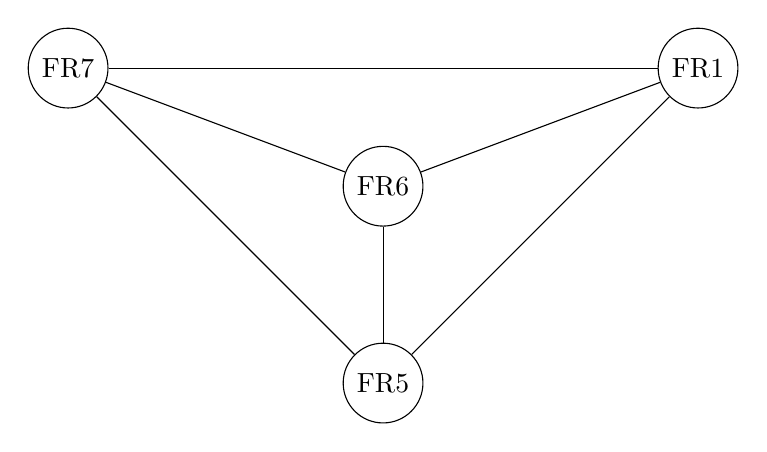
\begin{tikzpicture}
        \node [draw,circle] (fr1) at (4,0) {FR1};
        \node [draw,circle] (fr5) at (0,-4) {FR5};
        \node [draw,circle] (fr6) at (0,-1.5) {FR6};
        \node [draw,circle] (fr7) at (-4,0) {FR7};
        \draw (fr1) edge (fr5);
        \draw (fr1) edge (fr6);
        \draw (fr1) edge (fr7);
        \draw (fr5) edge (fr6);
        \draw (fr5) edge (fr7);
        \draw (fr6) edge (fr7);
      \end{tikzpicture}
    }

    \bigskip

    \(G_1-\text{FR4}-\text{FR3}\)
  \end{center}
  \caption{Design 1---Remove FR4 and FR3}
\end{figure}

At this point, \(G_1=K_4\), so it is guaranteed to fail the maximum edge threshold check for \(k=3\) and thus not
be \colorable{3}.  At \(k=4\) we have \(n=4\le4=k\).  Thus, we can conclude that \(G_1\) is \chromatic{4}. An
example chromatic coloring with:
\[C=\set{\text{\textcolor{green}{green}},\text{\textcolor{blue}{blue}},\text{\textcolor{red}{red}},
  \text{\textcolor{yellow}{yellow}}}\]
is show in Figure \ref{fig:d1color}.

\begin{figure}[h]
  \label{fig:d1color}
  \begin{center}
    \scalebox{0.75}{
      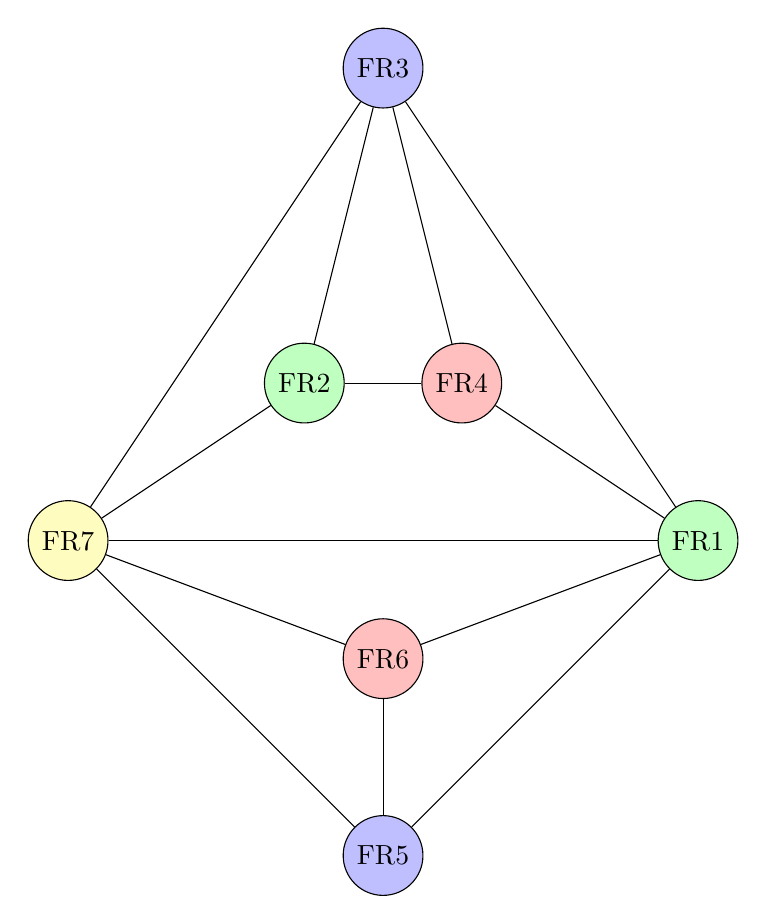
\begin{tikzpicture}
        \colorlet{c1}{green!25!white}
        \colorlet{c2}{blue!25!white}
        \colorlet{c3}{red!25!white}
        \colorlet{c4}{yellow!25!white}
        \node [draw,circle,fill=c1] (fr1) at (4,0) {FR1};
        \node [draw,circle,fill=c1] (fr2) at (-1,2) {FR2};
        \node [draw,circle,fill=c2] (fr3) at (0,6) {FR3};
        \node [draw,circle,fill=c3] (fr4) at (1,2) {FR4};
        \node [draw,circle,fill=c2] (fr5) at (0,-4) {FR5};
        \node [draw,circle,fill=c3] (fr6) at (0,-1.5) {FR6};
        \node [draw,circle,fill=c4] (fr7) at (-4,0) {FR7};
        \draw (fr1) edge (fr3);
        \draw (fr1) edge (fr4);
        \draw (fr1) edge (fr5);
        \draw (fr1) edge (fr6);
        \draw (fr1) edge (fr7);
        \draw (fr2) edge (fr3);
        \draw (fr2) edge (fr4);
        \draw (fr2) edge (fr7);
        \draw (fr3) edge (fr4);
        \draw (fr3) edge (fr7);
        \draw (fr5) edge (fr6);
        \draw (fr5) edge (fr7);
        \draw (fr6) edge (fr7);
      \end{tikzpicture}
    }

    \bigskip

    \(G_1\)
  \end{center}
  \caption{Design 1---Chromatic Coloring}
\end{figure}

Notice in the design that FR5 (start toasting) and FR6 (stop toasting) have been forced into separate parts,
conceivably to accommodate the separate ``cancel'' button shown in Figure \ref{fig:toaster}.  But what if the
designer decides to eliminate the cancel button and allow manual cancellation via the lever?  Thus, FR5 and FR6
no longer need to be separated, so the edge between their vertices can be eliminated.  The result is shown in Figure
\ref{fig:design2}.

\begin{figure}[h]
  \label{fig:design2}
  \begin{center}
    \scalebox{0.75}{
      \begin{tikzpicture}
        \node [draw,circle] (fr1) at (4,0) {FR1};
        \node [draw,circle] (fr2) at (-1,2) {FR2};
        \node [draw,circle] (fr3) at (0,6) {FR3};
        \node [draw,circle] (fr4) at (1,2) {FR4};
        \node [draw,circle] (fr5) at (0,-4) {FR5};
        \node [draw,circle] (fr6) at (0,-1.5) {FR6};
        \node [draw,circle] (fr7) at (-4,0) {FR7};
        \draw (fr1) edge (fr3);
        \draw (fr1) edge (fr4);
        \draw (fr1) edge (fr5);
        \draw (fr1) edge (fr6);
        \draw (fr1) edge (fr7);
        \draw (fr2) edge (fr3);
        \draw (fr2) edge (fr4);
        \draw (fr2) edge (fr7);
        \draw (fr3) edge (fr4);
        \draw (fr3) edge (fr7);
        \draw (fr5) edge (fr7);
        \draw (fr6) edge (fr7);
      \end{tikzpicture}
    }

    \bigskip

    \(G_2\)
  \end{center}
  \caption{Second Candidate Design}
\end{figure}

Rerun the algorithm on \(G_2\) for \(n=7\) and \(m=12\).  For \(k=2\), the maximum edge threshold test passes:
\[\frac{n^2(k-1)}{2k}=\frac{7^2(2-1)}{2\cdot2}=\frac{49}{4}\approx12.3>12=m\]
Note that \(N(\text{FR6})\subseteq N(\text{FR5})\), so remove FR6.  The result is shown in Figure \ref{fig:d2rem6}.

\begin{figure}[h]
  \label{fig:d2rem6}
  \begin{center}
    \scalebox{0.75}{
      \begin{tikzpicture}
        \node [draw,circle] (fr1) at (4,0) {FR1};
        \node [draw,circle] (fr2) at (-1,2) {FR2};
        \node [draw,circle] (fr3) at (0,6) {FR3};
        \node [draw,circle] (fr4) at (1,2) {FR4};
        \node [draw,circle] (fr5) at (0,-4) {FR5};
        \node [draw,circle] (fr7) at (-4,0) {FR7};
        \draw (fr1) edge (fr3);
        \draw (fr1) edge (fr4);
        \draw (fr1) edge (fr5);
        \draw (fr1) edge (fr7);
        \draw (fr2) edge (fr3);
        \draw (fr2) edge (fr4);
        \draw (fr2) edge (fr7);
        \draw (fr3) edge (fr4);
        \draw (fr3) edge (fr7);
        \draw (fr5) edge (fr7);
      \end{tikzpicture}
    }

    \bigskip

    \(G_2-\text{FR6}\)
  \end{center}
  \caption{Design 2---Remove FR6}
\end{figure}

Now, with \(n=6\) and \(m=10\), \(G_2\) fails the maximum edge threshold test for \(k=2\):
\[\frac{n^2(k-1)}{2k}=\frac{6^2(2-1)}{2\cdot2}=\frac{36}{4}=9<10=m\]
so \(G_2\) is not \colorable{2}.

For \(k=3\), note that \(\deg(\text{FR5})=2<3=k\), so remove FR5.  The result is shown in Figure \ref{fig:d2rem5}.

\begin{figure}[h]
  \label{fig:d2rem5}
  \begin{center}
    \scalebox{0.75}{
      \begin{tikzpicture}
        \node [draw,circle] (fr1) at (4,0) {FR1};
        \node [draw,circle] (fr2) at (-1,2) {FR2};
        \node [draw,circle] (fr3) at (0,6) {FR3};
        \node [draw,circle] (fr4) at (1,2) {FR4};
        \node [draw,circle] (fr7) at (-4,0) {FR7};
        \draw (fr1) edge (fr3);
        \draw (fr1) edge (fr4);
        \draw (fr1) edge (fr7);
        \draw (fr2) edge (fr3);
        \draw (fr2) edge (fr4);
        \draw (fr2) edge (fr7);
        \draw (fr3) edge (fr4);
        \draw (fr3) edge (fr7);
      \end{tikzpicture}
    }

    \bigskip

    \(G_2-\text{FR5}\)
  \end{center}
  \caption{Design 2---Remove FR5}
\end{figure}

Now, with \(n=5\) and \(m=8\), \(G_2\) passes the maximum edge threshold test for \(k=3\):
\[\frac{n^2(k-1)}{2k}=\frac{5^2(3-1)}{2\cdot3}=\frac{50}{6}\approx8.3>8=m\]
Since \(N(\text{FR2})\subseteq N(\text{FR1})\), remove FR2.  The result is shown in Figure \ref{fig:d2rem2}.

\begin{figure}[h]
  \label{fig:d2rem2}
  \begin{center}
    \scalebox{0.75}{
      \begin{tikzpicture}
        \node [draw,circle] (fr1) at (4,0) {FR1};
        \node [draw,circle] (fr3) at (0,6) {FR3};
        \node [draw,circle] (fr4) at (1,2) {FR4};
        \node [draw,circle] (fr7) at (-4,0) {FR7};
        \draw (fr1) edge (fr3);
        \draw (fr1) edge (fr4);
        \draw (fr1) edge (fr7);
        \draw (fr3) edge (fr4);
        \draw (fr3) edge (fr7);
      \end{tikzpicture}
    }

    \bigskip

    \(G_2-\text{FR2}\)
  \end{center}
  \caption{Design 2---Remove FR2}
\end{figure}

Finally, \(\deg(\text{FR4})=\deg(\text{FR7})=2<3=k\), so remove FR4 and FR7.  The result is shown in Figure
\ref{fig:d2rem47}.

\begin{figure}[h]
  \label{fig:d2rem47}
  \begin{center}
    \scalebox{0.75}{
      \begin{tikzpicture}
        \node [draw,circle] (fr1) at (4,0) {FR1};
        \node [draw,circle] (fr3) at (0,6) {FR3};
        \draw (fr1) edge (fr3);
      \end{tikzpicture}
    }

    \bigskip

    \(G_2-\text{FR4,FR7}\)
  \end{center}
  \caption{Design 2---Remove FR4 and FR7}
\end{figure}

This final state of \(G_2\) has \(n=2\le3=k\), so we can conclude that \(G_2\) is \chromatic{3}.  An example
chromatic coloring with:
\[C=\set{\text{\textcolor{green}{green}},\text{\textcolor{blue}{blue}},\text{\textcolor{red}{red}}}\]
is show in Figure \ref{fig:d2color}.
\begin{figure}[h]
  \label{fig:d2color}
  \begin{center}
    \scalebox{0.75}{
      \begin{tikzpicture}
        \colorlet{c1}{green!25!white}
        \colorlet{c2}{blue!25!white}
        \colorlet{c3}{red!25!white}
        \node [draw,circle,fill=c1] (fr1) at (4,0) {FR1};
        \node [draw,circle,fill=c1] (fr2) at (-1,2) {FR2};
        \node [draw,circle,fill=c2] (fr3) at (0,6) {FR3};
        \node [draw,circle,fill=c3] (fr4) at (1,2) {FR4};
        \node [draw,circle,fill=c2] (fr5) at (0,-4) {FR5};
        \node [draw,circle,fill=c2] (fr6) at (0,-1.5) {FR6};
        \node [draw,circle,fill=c3] (fr7) at (-4,0) {FR7};
        \draw (fr1) edge (fr3);
        \draw (fr1) edge (fr4);
        \draw (fr1) edge (fr5);
        \draw (fr1) edge (fr6);
        \draw (fr1) edge (fr7);
        \draw (fr2) edge (fr3);
        \draw (fr2) edge (fr4);
        \draw (fr2) edge (fr7);
        \draw (fr3) edge (fr4);
        \draw (fr3) edge (fr7);
        \draw (fr5) edge (fr7);
        \draw (fr6) edge (fr7);
      \end{tikzpicture}
    }

    \bigskip

    \(G_2\)
  \end{center}
  \caption{Design 2---Chromatic Coloring}
\end{figure}

This process gives the designer the feedback that the second design requires only three parts instead of four, and
thus has less information content and hence a higher chance of success than the first design.  It will be up to the
designer to weigh this result against other aspects of the design.


\bibliography{thesis}
\bibliographystyle{plain}

\end{document}
